\documentclass[12pt,a4paper,twoside]{scrartcl}

% Loading babel to enable automatic hypentation and multiple languages in the document.
% The last language in the option list will be used as default.
\usepackage[ngerman,english]{babel}
% Using T1 font encoding and the Latin Modern font
\usepackage[T1]{fontenc}
\usepackage{lmodern}
\usepackage{lscape}
\usepackage{afterpage}

% Using utf8 as file encoding.
\usepackage[utf8]{inputenc}
\usepackage[capbesideposition=outside,capbesidesep=quad]{floatrow}


% Page size. Using almost the whole A4 paper.
\usepackage[tmargin=22mm,bmargin=22mm,lmargin=20mm,rmargin=20mm]{geometry}


% Some standard packages for writing papers
\usepackage{latexsym,amsmath,amssymb,mathtools,textcomp}

% Paragraphs are not indented but there will be some space between paragraphs
\usepackage{parskip}
% For defining theorem-style environments like Lemma/Proof/Definition
\usepackage{amsthm}
% Fixing spacing problems before theorems due to \usepackage{parskip}
\begingroup
    \makeatletter
    \@for\theoremstyle:=definition,remark,plain\do{%
        \expandafter\g@addto@macro\csname th@\theoremstyle\endcsname{%
            \addtolength\thm@preskip\parskip
            }%
        }
\endgroup

% Some theorem-style environments
\newtheorem{theorem}{Theorem}[section]
\newtheorem{definition}[theorem]{Definition}
\newtheorem{lemma}[theorem]{Lemma}
% Setting equation numbers to <chapter>.<section>.<index>
\numberwithin{equation}{section}

% For inserting graphics into the document
\usepackage{graphicx}
\graphicspath{{images/}}

% For tables
\usepackage{array,multirow}

% Control layout of itemize, enumerate, description
\usepackage{enumitem}

\setlist[enumerate]{topsep=0pt}
\setlist[itemize]{topsep=0pt}
\setlist[description]{font=\normalfont,topsep=0pt}

\setlist[enumerate,1]{label=(\roman*)}

% TikZ for graphics in LaTeX
\usepackage{tikz}
\usetikzlibrary{calc}

% Have the current section and subsection in the header.
\usepackage{fancyhdr}
\usepackage{ltxtable} 
\fancypagestyle{plain}{
  \setlength\footskip{32pt}
  \fancyhead{}
  \fancyfoot{}
  \fancyfoot[LE,RO]{\normalsize\thepage}
  \renewcommand{\headrulewidth}{0pt}
  \renewcommand{\footrulewidth}{0pt}
}

\fancypagestyle{normal}{
  \setlength{\headheight}{20pt}
  \setlength\footskip{32pt}
  \fancyhead{}
  \fancyhead[LE]{\normalsize\textsc{\nouppercase{\leftmark}}}
  \fancyhead[RO]{\normalsize\textsc{\nouppercase{\rightmark}}}
  \fancyfoot{}
  \fancyfoot[LE,RO]{\normalsize\thepage}
  \renewcommand{\headrulewidth}{0.4pt}
  \renewcommand{\footrulewidth}{0pt}
}

% Hyperref for hyperlinks und cross refs
\usepackage{color}
\usepackage{lscape}
\usepackage[pagebackref]{hyperref}
\usepackage[all]{hypcap}
\usepackage{pbox}
\DeclareOldFontCommand{\bf}{\normalfont\bfseries}{\mathbf}
\hypersetup{
  pdftitle={SAT Solving with distributed local search},
  pdfauthor={Guangping Li}, 
  pdfsubject={SAT solver, \emph{\textbf{SAT}},distributed local search}, 
  colorlinks=true,
  pdfborder={0 0 0},
  bookmarksopen=true,
  bookmarksopenlevel=1,
  bookmarksnumbered=true,
  linkcolor=black,
  %linkcolor=black,
  citecolor=black,
  urlcolor=black,
  filecolor=black,
  pdfpagemode=UseNone,
  unicode=true,
}

% Add the word "page" for pagebackref's in the bibliography.
\renewcommand*{\backreflastsep}{, }
\renewcommand*{\backreftwosep}{, }
\renewcommand*{\backref}[1]{}
\renewcommand*{\backrefalt}[4]{%
  \ifcase #1 %
No citations.% use \relax if you do not want the "No citations" message 
  \or
(Page #2).%
  \else
(Pages #2).%
  \fi%
}


% For importing graphics from subdirectories.
\usepackage{import}

% Referencing figures, etc.
\newcommand{\reflst}[1]{\hyperref[#1]{Listing~\ref*{#1}}}
\newcommand{\refthm}[1]{\hyperref[#1]{Theorem~\ref*{#1}}}
\newcommand{\refdef}[1]{\hyperref[#1]{Definition~\ref*{#1}}}




% Package for inserting pseudo codes in the document.
\usepackage[ruled,vlined,linesnumbered,norelsize]{algorithm2e}
\DontPrintSemicolon
\def\NlSty#1{\textnormal{\fontsize{8}{10}\selectfont{}#1}}
\SetKwSty{texttt}
\SetCommentSty{emph}
\def\listalgorithmcfname{List of Algorithms}
\def\algorithmautorefname{Algorithm}
\let\chapter=\section % resolve a problem with algorithm2e

\begin{document}

%%%%%%%%%%%%%%%%%%%%%%%%%%%%%%%%%%%%%%%%%%%%%%%%%%%%%%%%%%%%%%%%%%%%%%
\pagestyle{empty} % no page number
\pagenumbering{alph}

% title page
\begin{titlepage}

  \begin{center}\large

    {\flushleft
\includegraphics[height=17mm]{kit_logo_en.pdf} \hfill}
%    \includegraphics[height=20mm]{grouplogo-algo-blue.pdf}\quad\null

    \vfill

    \vspace*{2cm}

    {\bf\huge SAT Solving  \\ with distributed local search \par} 
    % Be sure to fill in the field pdftitle={} above
    % mit \par am Ende stimmt der Zeilenabstand
  

    \vfill
Master Thesis of \\

    \vspace*{15mm}
    {\bf Guangping Li} 

    \vspace*{15mm}

    At the Department of Informatics\\
Institute of Theoretical informatics, Algorithmics II 

    \vspace*{45mm}

    \begin{tabular}{rl}
      Advisors: & Dr. Tom{\' a}{\v s} Balyo \\
      & Prof. Dr. Peter Sanders  \\
    \end{tabular}
    
    \vspace*{10mm}

	% Deutsch
%    Institut für Theoretische Informatik, Algorithmik \\
%    Fakultät für Informatik \\
%    Karlsruher Institut für Technologie

    % English:
%     Institute of Theoretical Informatics, Algorithmics \\

    \vspace*{12mm}
  \end{center}
\afterpage{\null\newpage}
\end{titlepage}
\afterpage{\null\newpage}
%%%%%%%%%%%%%%%%%%%%%%%%%%%%%%%%%%%%%%%%%%%%%%%%%%%%%%%%%%%%%%%%%%%%%%
\vspace*{0pt}\vfill

\selectlanguage{ngerman}
\hrule\medskip

Hiermit versichere ich, dass ich diese Arbeit selbständig verfasst und keine anderen, als die angegebenen Quellen und Hilfsmittel benutzt, die wörtlich oder inhaltlich übernommenen Stellen als solche kenntlich gemacht und die Satzung des Karlsruher Instituts für Technologie zur Sicherung guter wissenschaftlicher Praxis in der jeweils gültigen Fassung beachtet habe.

\bigskip

\noindent
Karlsruhe, 20th September 2018 

% Hand-written signature!! %TODO

\vspace*{5cm}

\clearpage

%%%%%%%%%%%%%%%%%%%%%%%%%%%%%%%%%%%%%%%%%%%%%%%%%%%%%%%%%%%%%%%%%%%%%%

\vspace*{0pt}\vfill
\selectlanguage{english}
\begin{abstract}
\centerline{\bf Abstract}
{\noindent Stochastic local search (SLS) is an elementary technique for solving combinational problems. In the first section of this paper, we introduce an efficient SLS heuristic solver for Boolean Satisfiability Problem (SAT), in which the decisions only based on the probability distribution. We experimentally evaluate and analyze the performance of our solver in a combination of different techniques, including simulated annealing and walkSAT. With formula partition, we introduce a parallel version of our solver in the second section. The parallelism improves the efficiency of the solver. Using different random generator in solving
the sub-formula can bring further improvement in performance to our parallel solver.}
\end{abstract}
\vfill
\afterpage{\null\newpage}
\selectlanguage{ngerman}
\begin{abstract}
\centerline{\bf Zusammenfassung}
{\noindent Stochastische lokale Suche (SLS) stellt eine elementare Technik zur Lösung von komplizierten kombinatorischen Problemen dar. Im ersten Teil dieser Arbeit stellen wir eine effiziente SLS Heuristik für das Erfüllbarkeitsproblem der Aussagenlogik (SAT) vor, bei dem die Entscheidungen nur auf der Wahrscheinlichkeitsverteilung basieren. Die Leistung unseres Algorithmus in einer Kombination verschiedener Techniken, einschließlich simulierter Abkühlung und walkSAT, wurde auch experimentell bewertet und analysiert. Mit Formelpartition wird im zweiten Teil eine parallele Version unseres Algorithmus eingeführt, die die Effizienz des Solvers verbessert. Flexible Parametereinstellungen kann eine weitere Verbesserung unseres Algorithmus bringen.
 }
\end{abstract}


\vfill\vfill\vfill
\clearpage

%%%%%%%%%%%%%%%%%%%%%%%%%%%%%%%%%%%%%%%%%%%%%%%%%%%%%%%%%%%%%%%%%%%%%%

\selectlanguage{english}
\pagestyle{plain}
\pagenumbering{roman}
  
% markiere sections im Seitenkopf links und subsections rechts
\renewcommand\sectionmark[1]{\markboth{\thesection\quad\MakeUppercase{#1}}{\thesection\quad\MakeUppercase{#1}}}
\renewcommand\subsectionmark[1]{\markright{\thesubsection\quad\MakeUppercase{#1}}}


\tableofcontents
\afterpage{\null\newpage}
\clearpage

%%%%%%%%%%%%%%%%%%%%%%%%%%%%%%%%%%%%%%%%%%%%%%%%%%%%%%%%%%%%%%%%%%%%%%
%%%%%%%%%%%%%%%%%%%%%%%%%%%%%%%%%%%%%%%%%%%%%%%%%%%%%%%%%%%%%%%%%%%%%%
\pagestyle{normal}
\pagenumbering{arabic}

\section{Introduction} 
\label{sec:Intro}
\subsection{Problem/Motivation} 
The \emph{\textbf{propositional satisfiability problem}} (\emph{\textbf{SAT}}) is the first proven NP-complete problem\cite{cook1971complexity}. The problem is to determine whether an assignment of boolean values to variables in a boolean formula exsits such that the expression evaluates to true. Hard combinational problems can be resolved with appropriate encoding as a SAT problem.
The SAT problem has many applications in computer science like chip model checking\cite{clarke2001bounded}, software verification\cite{ivanvcic2008efficient} or in automated planning and scheduling in artificial intelligence\cite{kautz1999unifying}. \\
Formula partition is one of the promising approaches in DPLL-like solvers\cite{mann2017guiding}. By prioritizing the variables according to a good formula partition, the search gets a relatively balanced decision tree. But formula partition is rarely used in a local search for the SAT problem. Questions such as how to combine the formula partition with local search, whether the local search can benefit from the partition, and whether the formula partition can guide a parallel local search still remain open. 

\subsection{Content} 
The SAT problem, as a well-known NP-complete problem, has drawn remarkable attention and different local search heuristics have been developed to tackle this problem. In this thesis, we introduced a stochastic local search on SAT problem using formula partition as guidance. \\
In section~\ref{sec:Intro}, we summarized the formal concept and techniques used in this thesis. Section~\ref{sec:local} described our method which is a combination of  \emph{probSAT} and \emph{walkSAT}. Then we  discussed some attempts at improving the algorithm. By experimental evaluation and comparison, some techniques turned out to be more efficient than the simple \emph{probSAT} search. In section~\ref{sec:parallel}, we inspected the potential benefit of formula partition in a parallel search. Section~\ref{sec:eva} described the experiments mentioned in section~\ref{sec:local} and section~\ref{sec:parallel} with details and empiric results.  Section~\ref{sec:conc} concluded our work based on the experiments, alongside a discussion of some limitations of our solver and further work. 

\subsection{Definitions and Notations} 
\emph{\textbf{Propositional Satisfiability Problem}}\\
A variable with only two possible logical values  \textit{true} or  \textit{false} is a \emph{\textbf{propositional variable}}, which will be referred to as \emph{\textbf{variable}} in this thesis.     \\
A \emph{\textbf{literal}} is an atomic formula in propositional logic. A literal can either be a \emph{\textbf{positive literal}} $v$ as the variable $v$ or a \emph{\textbf{negative literal}} $\bar{v}$ as negation of $v$.\\
A \emph{\textbf{clause}} is a disjunction of literals. A formula in conjunctive normal form (CNF) is a conjunction of clauses. We refer it as  \emph{\textbf{CNF-formula}} or simply as \emph{\textbf{formula}} in this thesis.\\
An \emph{\textbf{assignment}} $a$: $V\rightarrow \{true {, }\; false\}$ assigns a truth value to each variable $v$ in the formula. An assignment satisfies a formula if the truth value of the formula with this assignment evaluates to true. Specifically, an assignment satisfies a clause, if at least one literal in the clause is assigned with value  \textit{true}. \\
An assignment $a$ is a satisfying assignment if it  satisfies all clauses in the formula. Otherwise, there are conflicts in some clauses with this assignment, or some clauses are unsatisfied clauses with this assignment. 
A \emph{\textbf{satisfiable formula}} is a formula which can be satisfied by some assignment. The SAT problem is to determine whether a given formula is satisfiable or not.  \\
\\
Here is an example of SAT problem:
\begin{center}tau
\begin{table}[H]
\begin{tabular}{l}
$F = (v_1 \lor \bar{v_3}) \land (v_2 \lor v_1 \lor \bar{v_1})$\\	
$Vars(F) = \{v_1, v_2, v_3\}$\\
$\emph{numV}(F) = |Vars(F)| = 3$\\
$Lits(F) = \{v_1, \bar{v_1}, v_2, v_3, \bar{v_3}\}$\\
$Cls(F) = \{C_1, C_2\}$\\
$numC(F) = |Cls| = 2$\\ 
$C_1 = \{v_1, \bar{v_3}\}$\\
$C_2 = \{v_2, v_3, \bar{v_1}\}$\\
\\
$A(v_1)$ = $true$, $A(v_2)$ = $false$, $A(v_3)$ = $true$, \\
$A$  is an assignment satisfying $F$.\\
\\
$\hat{A}(v_1)$ = $true$, $\hat{A}(v_2)$ = $false$, $\hat{A}(v_3)$ = $false$, \\
$\hat{A}$  is an assignment with conflict in $C_2$.\\
\\
\end{tabular}
\label{table:kysymys}
\end{table}
\end{center}




\emph{\textbf{Set}}\\
A set is a container of unique elements. A set of three objects $ a, b, c$ is written as $\{a, b, c\}$. The
size of a set is the number of elements in the set.


\emph{\textbf{Local Search}}\\
For an instance $I$ of a hard combinational Problem $P$, there is a set of solutions $S(I)$. An object function (score or cost) $\Gamma$ is derived from the constraints of the problem to evaluate the candidate solutions. The goal of the local search is to find the solution with minimum cost ( or the solution with maximal score).\\
A local search starts with an initial complete solution. According to some heuristic, the local search makes local changes to its current solution iteratively, hence the name \emph{\textbf{local search}}. Starting from an initial solution, the search will evaluate the neighbor solutions which are reached by applying a local change to the current solution and choose one of the neighbor solutions with local optimization. The search applies local moves until the optimal solution is reached, or in some cases, a generally good solution is reached.  Local search is widely used in hard combinational problems such as the traveling salesman problem\cite{johnson1990local} and the graph coloring problem\cite{galinier2006survey}. \\
\\
\emph{\textbf{Local Search in SAT Problem}}\\
In the boolean satisfiability problem, a local search operates primarily as follows: The search starts from a randomly generated assignment as the initial solution. If this current assignment satisfies the formula, the search stops with success. Otherwise, a variable is chosen depending on some criterion. This selection is called \emph{\textbf{pickVar}}. By changing the assignment of the selected variable $v$, a neighbor assignment $\hat{A}$ of our current solution $A$ is reached in next step. The move is also called  \emph{\textbf{flip$(A,v)$}}. A local search will move in the space of the assignments by flipping the variables until a satisfying assignment is reached by the search. \\
The heuristic used for \emph{pickVar}  is based on scores of the variables in the current assignment. Consider the assignment $\hat{A}$  reached by taking a flip of the variable in the current assignment $A$. The number of clauses satisfied in $A$, but not in $\hat{A}$ is called the \emph{\textbf{breakcount}} of the local move from $A$ to $\hat{A}$. Accordingly, the number of clauses which become satisfied because of the flipping, is the  \emph{\textbf{makecount}}. The number of newly satisfied clauses ($makecount$) minus the number of newly unsatisfied clauses ($breakcount$), which is denoted as \emph{\textbf{diffscore}}, represents the local improvement of the corresponding flipping. Apart from this, other aspects such as the repetition number of each flip or the number of occurrences of the variables can be included in a selection heuristic. An example is the local solver \emph{EagleUp}, which prefers flipping of variables with the highest number of occurrences in the formula to create new unit clauses for unit propagation. To get local improvement effectively, it is sufficient to only consider variables in unsatisfied clauses for the flipping selection. This commonly used process is called a \emph{\textbf{focused local search}}. \\
\\
\begin{algorithm}[h!]
\SetKwInOut{Input}{input}
\SetKwInOut{Output}{output}
\SetKwInOut{Parameter}{parameter}
 \Input{A CNF Formula F}
 \Parameter{$Timeout$}
 \Output{a satisfying assignment $A$}
  $A \leftarrow$ random generated assignment  $A$;\;
 \While {$( \exists$ unsatisfied clause $ \land$ Timeout does not occur$)$}{
  $c \leftarrow$ random selected  unsatisfied clause ;\;
  $x \leftarrow pickVar(A,c)$\;
  $A \leftarrow flip(A,x)$;\;
 }
 \caption{Focused Local Search}
\end{algorithm}  

By choosing the variable with best score in \emph{pickVar}, the search will get greedy local improvement. 
The initial intention of the local search is that the optimal global solution can be found through iterative greedy local improvement. The typical problem of the local search is that the greedy moves can be trapped in local optimal solutions, which are however not global optimums. To avoid this, some random flips are picked or even a worse solution  will be chosen for the next step (\emph{\textbf{uphill moves}}). The following techniques are commonly used to prevent local search from getting stuck in local regions.

\emph{\textbf{Stochastic Local Search (SLS)}}\\
The stochastic local search will use the probability distribution of the scores of candidate solutions instead of the static decision. For the candidate moves, the probability of being chosen $p(\Gamma(s))$ corresponds to the score $\Gamma(s)$ of the solution $s$. In this way, the more advantageous a move is, the higher is the probability of choosing that move as the next step. This randomization can help the search get rid of cycling and decrease the chance of getting misled by specific heuristics.\\
\\
\emph{\textbf{Statistical Local Search }}\\
 Tabu search was proposed by Fred W. Glover in 1986 and formalized in 1989\cite{glover1989tabu}. To recognize the loops in suboptimal region, the recent search moves are marked as tabu moves. These tabu moves will not be touched in the further search to discourage getting stuck in a region. Inspired by the tabu search, a statistical search will record the whole search trace, in which the number of times each variable is chosen for flipping are counted. Through the use of the statistical information, the search will prefer the variables with fewer flippings before. We have experimentally verified that a statistical search can recognize short-term cyclings like tabu search and permit long-term cyclings\cite{lisolving}.\\
\\
\emph{\textbf{Simulated Annealing}}\\
Simulated Annealing is an approach of local search solver to difficult combinational optimization problems proposed by Kirkpatrick, Gelatt, and Vecchi\cite{kirkpatrick1983optimization}. This approach is inspired by the metallic process annealing, in which material is shaped by heating and then slowly cooling. This approach works as a local optimization algorithm guided by a controlling parameter \emph{\textbf{temperature}}. Higher temperature allows uphill moves with higher probability. The temperature varies according to the score of the current situation.  For a current solution with a nearly optimal score, the temperature is nearly zero. For an unattractive local extreme with a poor score, the active search tends to make uphill moves due to high temperature.\\
\\
\emph{\textbf{walkSAT}}\\
The focused random local search strategy \emph{walkSAT} to solve SAT problem, which is originally introduced in 1994\cite{hoos2002adaptive}. The \emph{walkSAT} may ignore the greedy flipping and flip a random variable in a chosen unsatisfied clause with probability $p$ . By introducing these ``uphill noises'', the walkSAT combines greedy local search and random walk to get an effective and robust random solver. \\
\\
\begin{algorithm}[H]
\SetKwInOut{Input}{input}
\SetKwInOut{Output}{output}
\SetKwInOut{Parameter}{parameter}
 \Input{current assignment $A$, unsatisfied clause $c$}
 \Parameter{probability $p$}
 \Output{a variable $x$ in $c$ to be flipped}
\For{$v$ in $c$}{
  Evaluate $v$ with function $\Gamma(A,v)$;\;
 }
  with probability $p$: $x \leftarrow$   $v$ with maximum $\Gamma(A,v)$; \;
  with probability $1-p$:  $x \leftarrow$  randomly selected $v$ in $c$. 
 \caption{pickVar in WalkSAT}
\end{algorithm}  

\emph{\textbf{The probSAT}}\\
The SLS solver \emph{probSAT} was introduced in 2012 by Adrian Balint and Uwe Schoening\cite{balint2016engineering}. In a \emph{probSAT} solver, the score of a candidate flip is solely based on the make- and breakcount. The paradigm is as follows: Firstly, a completely random assignment is set as the initial assignment. Then the algorithm performs local moves by flipping a variable in a random chosen unsatisfied clause and stops as soon as there exists no unsatisfied clause, which means a satisfying assignment is found. The probability $p(v)$ of flipping the variable $v$ in the chosen clause is proportional to the score of $v$, which is calculated by the function $\Gamma(v,A)$ based on breakcount of $v$ in the current assignment $A$.\footnote{As mentioned in the \emph{probSAT} paper, the influence of makecount is rather weak in selection functions in experiments.} 
\\
 \\ There are two kinds of score functions in the paper by Adrian Balint: \\
\begin{center}
$\Gamma(v,A) = (c_b)^{-break(v,A)}$ (break-only-exp-function) \\
$\Gamma(v,A)=(\epsilon +break(v,A)^{-c_b})$  (break-only-poly-function)\\
\end{center} 
\clearpage
The pseudocode of \emph{probSAT} is shown below:\\
\begin{algorithm}[H]
\SetKwInOut{Input}{input}
\SetKwInOut{Output}{output}
\SetKwInOut{Parameter}{parameter}
 \Input{current assignment $A$, unsatisfied clause $c$}
 \Output{a variable $x$ in $c$ to be flipped}
\For{$v$ in $c$}{
  Evaluate $v$ with function $\Gamma(A,v)$;\;
 }
  $x \leftarrow$ randomly selected  variable $v$ in $c$ with probability $p(v) =\frac{\Gamma(A,v)}{\sum_{u \in c}\Gamma(A,u)}$; 
 \caption{pickVar in \emph{probSAT}}
\end{algorithm} 
\emph{\textbf{Formula partition}}\\
To introduce our parallel SAT solver with formula partitioning, we use a  hypergraph representation of the SAT problem. \\
A hypergraph $G = (V,H)$ is a generalized graph, in which a hyperedge $h \in H$ is a non-empty subset of the vertices set $V$. For a SAT formula $F$, its hypergraph representation $G(F)$ = (\emph{Vars}(\emph{F}), \emph{Cls}(\emph{F})) consists of \emph{numV} vertices and \emph{numC} hyperedges. 
  Each vertex corresponds to a variable in $F$, and a hyperedge refers to a clause, which connects the variables in this clause. \\
\\
Here is an example:\\
$F =\underbrace{(v_1 \lor v_2 \lor \bar{v_3})}_\text{$C_1$} \land \underbrace{(v_1 \lor v_3\lor \bar{v_4})}_\text{$C_2$}\land \underbrace{(v_5 \lor v_6\lor \bar{v_8})}_\text{$C_3$}\land \underbrace{(v_6 \lor v_7\lor \bar{v_8})}_\text{$C_4$}\land \underbrace{(v_3\lor \bar{v_6})}_\text{$C_5$}\land \underbrace{(v_4 \lor v_5)}_\text{$C_6$}$\\
$G(F)$:
\begin{figure}[H]
\begin{center}
  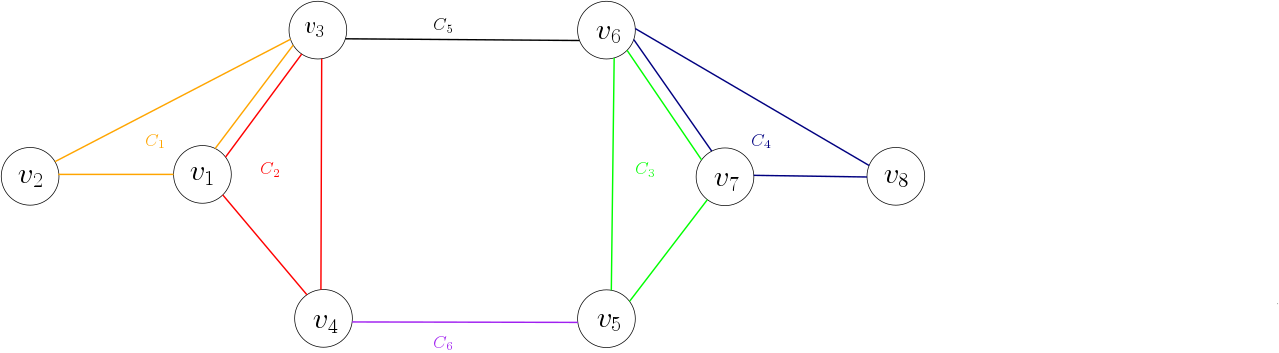
\includegraphics[scale = 0.4]{1/hypergraph.png}
  \end{center}
  \caption{In a hypergraph, a hyperedge is a set of vertices. In this example, the vertices  $v_3$  and $v_4$ are in both hyperedge $\{v_1, v_3, v_4\}$ and $\{v_1, v_2, v_3\}$, so they are connected twice. In our hypergraph representation, a hyperedge contains the vertices of the corresponding clauses. In another variant, each literal refers to one vertex and a hyperedge contains all the literals of the corresponding clause.}
  \label{hypergraph representation}
  \end{figure}

Formula partition is a promising way to improve the SAT problem solving. Two partitioning have already been well investigated. One is to divide the variables, which is used in this thesis, and another one is to separate the clauses. For algorithms with the technique of decision tree like \emph{DPLL}\cite{nieuwenhuis2005abstract}, the formula partition can be used to prioritize decisions. For the local search, there is scarce research using formula partition in local search. Based on hypergraph represenation, we describe the formula partition with the notations of graph partition in this thesis. For a hypergraph $G = (V,H)$,  a two-way partitioning is to seperate the vertices in two disjoint subsets $P_0$ and $P_1$.  Based on the partitioning of vertices, the hyperedges are seperated in three disjoint subsets $H_0$, $H_1$ and $I$. $H_0$ contains the edeges connecting verticse in $P_0$, $H_1$ are edges in $P_1$. The \textbf{intersection} $I$ are the edges containing vertices in $P_0$ and vertices in $P_1$. In a good balanced partition, $P_0$ and $P_1$ are relatively of the same size and only few edges are in the intersection. In our example formula above, a minimum cost balanced partition is $P_0$ = $\{v_1,v_2, v_3, v_4\}$ and $P_1$ = $\{v_5,v_6, v_7, v_8\}$. In this partition, $H_0$ = $\{C_1,C_2\}$ , $H_1$ = $\{C_4,C_5\}$ and the intersection $I$ = $\{C_5,C_6\}$ 
\subsection{The Competitors}
\label{comparision}
Our heuristic is based on the \emph{probSAT} paradigm. To evaluate the performance of our algorithm, we compare our heustic with the original \emph{probSAT}. Another competitor is \emph{yalSAT}, which is the champion in random track category of the SAT competition 2017\cite{biere2014yet}.\\
\\
\emph{\textbf{probSAT}} 
\\
The authors of the original paper implemented the \emph{probSAT}.\footnote{https://github.com/adrianopolus/probSAT} We compare our solver with the original implemen.\footnote{Using same parameter settings our implementation gets similar performance to the original code}  \\
Two implementation variants are available. In the incremental approach, the breakcounts of variables are calculated in the initialization phase and only updated in the further search. The other straightforward approach is to compute scores of the variables in chosen clauses on the fly. This method is called non-incremental approach in original paper. To get optimal results of the \emph{probSAT} solver, we take the non-incremental approach to the 3SAT problems and incremental method for 5SAT and 7SAT.\\
The parameters of \emph{probSAT} in our experiments have been set as suggested in the original paper:\\
\begin{table}[h!]
%\begin{minipage}{\textwidth}                                                                                         
\begin{center}
    \begin{tabular}{| l | l| l | l| l |p{3cm}|}
\hline 
    $k$SAT & score $\Gamma$ & $c_b$ & $\epsilon$ &variants \\ \hline
    $3$SAT & break-only-poly& 2.06 & 0.9 &non-incrementel \\ \hline
    $5$SAT & break-only-exp & 3.7 & - & incremental \\ \hline
    $7$SAT &  break-only-exp & 5.4 & - & incremental \\ \hline
\end{tabular}
\caption[probSAT]{Parameter settings for competitor \emph{probSAT}}
\end{center}
%\end{minipage}
\end{table} 

\emph{\textbf{yalSAT}}\\
We use the third version of yalSAT submitted to the 2017 SAT competition in our experiments. Armin Biere implements it as a reimplementation of \emph{probSAT}  with extensions.\footnote{https://baldur.iti.kit.edu/sat-competition-2017/solvers/random/}  The yalSAT uses a variant of \emph{probSAT} randomly in the restart of a searchround. In our comparison, we use the default settings of the yalSAT with specific seeds (See ~\ref{sec:seed}).
\clearpage
\section{Our local Solver}
\label{sec:local}
 Our algorithm is a typical focused SLS algorithm, which solves the SAT problem with the basic schema:\\
\\
\begin{algorithm}[H]
\SetKwInOut{Input}{input}
\SetKwInOut{Output}{output}
\SetKwInOut{Parameter}{parameter}
 \Input{A CNF Formula F}
 \Parameter{$Timeout$}
 \Output{a satisfying assignment $A$}
  $A \leftarrow initAssign(F)$ \;
 \While {$( \exists$ unsatisfied clause $ \land$ Timeout does not occur$)$}{
  $c \leftarrow pickCla(A)$ \;
  $x \leftarrow pickVar(A,c)$\;
  $A \leftarrow flip(A,x)$\;
 }
 \caption{Our Local Search}
\end{algorithm}
 In the following, we will describe the steps used in our local search.\\
\subsection{initAssign(F)}
In our algorithm, there are three variants to initialize assignment.
\emph{RandomInit} is the random initiation also used in the original \emph{probSAT}. The other two alternatives are \emph{BiasInit} and \emph{Bias-RandomInit}, which take the number of literal occurrences into consideration. With the method \emph{BiasInit} we assign \emph{true} to a variable if the number of occurrences of its positive literal is larger than that of its negative literal. Otherwise, a variable is initialized with \emph{false}. \emph{Bias-RandomInit} combines the two methods above by generating the assignment bias randomly based on the occurrences of literals.  In Experiment 1 (see \ref{sec:Experiment 1}) we compare these three alternatives based on the \emph{probSAT} algorithm. Our local search uses \emph{RandomInit} for 3SAT problems and \emph{BiasInit} for the other problems.\\
\\
\subsection{pickCla(A)}
The number of \emph{true} values in each clause $c$, \emph{numT}(\emph{c}) , are counted in Initilization phase and maintained in further search. During the local flipping, these numbers will be updated for clauses containing the flipping variable (See~\ref{subsec:Data structures}).  Unsatisfied clauses will be stored in a set \emph{UNSAT}. Compared to \emph{numT}, \emph{UNSAT} is updated  ``lazily''. After flipping, if \emph{numT} of one clause is decreased to zero, the clause will be added to \emph{UNSAT}.  To select an unsatisfied clause in $pickCla(A)$, one needs to select a clause from \emph{UNSAT} and check if it is still unsatisfied with its $numT$ being zero. Otherwise, if the chosen clause $c$ with $numT(c)$ as zero, it will be removed from \emph{UNSAT} set. This step $pickCla(A)$ will be repeated until one unsatisfied clause is found.\\ 
\\
\subsection{pickVar(A,c)}
Inspired by \emph{probSAT} and \emph{walkSAT}, our \emph{pickVar} combines the random walk and stochastic selection. 
The selection procedure in \emph{probSAT} is a random heuristic. Judging from the experiments, even if the search is very close to a satisfying assignment, and the probability of the critical flipping is exceptionally high, it is still possible that the stochastic search make uphill moves and leave the region of the global minimum. To prevent this,  we pick greedy flips with zero breakcounts with a certain probability $p$. With probability ($1-p$), we choose the variable to be flipped using the \emph{probSAT} heuristic.\\
\\
\begin{algorithm}[H]
\SetKwInOut{Input}{input}
\SetKwInOut{Output}{output}
\SetKwInOut{Parameter}{parameter}
 \Input{current assignment $A$, unsatisfied clause $c$}
 \Parameter{probability $p$}
 \Output{a variable $x$ in $c$ to be flipped}
 \emph{greedyVs} $\leftarrow$ $\emptyset$;\;
\For{all $v$ in $c$}{
   \If{$($break(A,v)= 0 $)$}{
	\emph{greedyVs} = \emph{greedyVs} +  $\{v\}$    
   }
 }
  with probability $p$: $x \leftarrow$ randomly selected variable $v \in$ \emph{greedyVs};  \;
  with probability ($1-p$):   $x \leftarrow$ randomly selected  variable $v$ in $c$ with probability $\frac{\Gamma(A,v)}{\sum_{u \in c}\Gamma(A,u)}$;  
\caption{Our pickVar}
\end{algorithm}  
We analyze the following variants for  \emph{pickVar} experimentally (see experiment in~\ref{sec:Experiment 2}).\\
\\ 
 \emph{\textbf{Variant 1: WALK}}\\
\\
Instead of using a constant probability $p$ to choose between a greedy literal without clause break and the random literal using \emph{probSAT} selection directly, we use a statistic list $S$ to record how many times each variable is chosen for flipping. To avoid cycling, the variable $v_i$ with a high value of $S[i]$ is used for flipping with low probability. After selecting a greedy literal and a variable using the \emph{probSAT} stochastic distribution, we make the choice randomly according to the statistic values of these two variables.\\
 \\
\begin{algorithm}[H]
\SetKwInOut{Input}{input}
\SetKwInOut{Output}{output}
\SetKwInOut{Parameter}{parameter}
 \Input{current assignment $A$, unsatisfied clause $c$}
 \Parameter{probability $p$}
 \Output{a variable $x$ in $c$ for flipping}
 greedyVs $\leftarrow$ $\emptyset$;\;
\For{all $v$ in $c$}{
   \If{$($break(A,v)= 0$)$}{
	greedyVs = greedVs +  $\{v\}$    
   }
 }
  $greedyV \leftarrow$   randomly selected variable $v \in$ greedyVs  ; \;
  $randomV \leftarrow$ randomly selected  variable $v$ in $c$ with probability $\frac{\Gamma(A,v)}{\sum_{u \in c}\Gamma(A,u)}$;  \;
  with probability $p = \alpha \times \frac{s(greedyV)}{s(greedyV)+s(randomV)}$: $x\leftarrow$ randomV;\;
    with probability $1-p$: $x\leftarrow$ greedyV;\;
\caption{WALK}
\end{algorithm} 
\clearpage
 \emph{\textbf{Varinat 2: GreedyBreak}}\\
\\ Getting a random literal using stochastic process consumes the most runtime in the search. In this variant \emph{GreedyBreak}, we search for greedy literals with small statistic values. A literal is treated as  a \emph{permitted greedy literal} if its breakcount is zero and its statistic value is under a certain threshold. If one permitted greedy literal exists, we choose it for flipping. If multiple permitted greedy literals exist, we choose one randomly for flipping. Otherweise, we pick a literal using \emph{probSAT} heuristic.\\ To set the threshold based on the search history, we compare two functions in our experiment. In the first approach \emph{Average}, the threshold is set to $\alpha \times \frac{numF}{numV}$. Here the \emph{numF} represents the number of flips. In another approach \emph{Random-Flip}, we select  a value $r $ randomly in $[0,$  \emph{numF}]. For each greedy literal, we check if its statistic value is smaller than $\alpha \times r$. \\
\\
\begin{algorithm}[H]
\SetKwInOut{Input}{input}
\SetKwInOut{Output}{output}
\SetKwInOut{Parameter}{parameter}
 \Input{current assignment $A$, unsatisfied clause $c$}
 \Parameter{probability $p$}
 \Output{a variable $x$ in $c$ for flipping}
  \emph{greedyVs} $\leftarrow$ $\emptyset$;\;
\For{all $v$ in $c$}{
   \If{$($break(A,v)= 0 $\land$ $Permit(v))$}{
	 \emph{greedyVs} =  \emph{greedyVs} + $\{v\}$   
   }
 }
  \If{$($greedyVs is not empty$)$}{
  		 x $\leftarrow$ selected variable $v$ in  \emph{greedyVs} randomly 
 	}
 \Else{
  x $\leftarrow$ randomly selected  variable $v$ in $c$ with probability $\frac{\Gamma(A,v)}{\sum_{u \in c}\Gamma(A,u)}$}
  \;
\caption{GreedyBreak}
\end{algorithm} 
\subsection{pickVar(A,c) with simulated annealing}
\emph{Simulated annealing} is a technique, whose combination with \emph{walkSAT} is extensively studied. Besides the dynamic noises introduced above, we use \emph{simulated annealing} to improve our three suggestions of \emph{pickVar}. That is, we define the parameter $\alpha$ as a function of two parameters tolerence $\tau$, $c_b$ and the quality function of current assignment $q(A)$ instead of using a static parameter in the whole process:
\begin{center}
 $\alpha = \tau \times (c_b)^{-q(A)}$\\
 \end{center}
To define the quality function $q(A)$, we have two variants: \emph{Global} and \emph{Local}.\\
\textbf{Global}:\\
In the process of search, the number of unsatisfied clauses is stored in $unsatN$. In the variant $Global$, we use this number to define the quality of the current solution:
\begin{center}
 $q_{global}(A) =unsatN(A)$.\\
\end{center}
\textbf{Local}:
As suggested by the name, in the $Local$ variant, we measure the quality of the current assignment focused on the chosen clause $c$. The quality  $q(A,c)$ is equal to the number of greedy literals in current clause:
\begin{center}
 $q_{local}(A) =|\{ v| v \in  c \land break(v) = 0\}|$\\
 \end{center}
\subsection{Data structures}
\label{subsec:Data structures}
In this section, the data structure of our SAT solver is introduced. \\
\emph{\textbf{Occurrences}}
\\
In the process of initialization, the numbers of positive and negative occurrences of one variable will be compared. In our implementation, we use a list to count and record these numbers of occurrences. This list of size $2 \times numC $ is denoted as \emph{occurrences list OL}. For the variable with index $i$, $OL[2i]$ is the number of occurrences of literal $v_i$; $OL[2i+1]$ is for its negative occurrences. \\
\\
\emph{\textbf{ Literals}}
\\
Only small changes are made in each step of local search. In our situation, only the clauses including the flipping variables are involved in the flipping step. To find the involved clauses of one variable,  two $2D$ array $posL$ and $negL$ are created to record the clauses of positive nad negative literals. For variable $v_i $, posL[i] records the indices of clauses containing the positive literal $v_i$. The ones with negative literal $\bar{v_i}$ are in $negL[i]$. We flip variable $v_i$ by updating the $numT$ of clauses with indices in $posL[i]$ and $negL[i]$.\\
\\
\emph{\textbf{LookUp}}
\\
The most time used in the search is the repeated  evaluation of the polynomial or exponential decay function $\Gamma$. We calculate the $\Gamma(x)$ with $x$ from $0$ to $0.5 \times numC$ and keep the values in a table $lookUp$. In our implementation, we use this table to get the values instead of the reputation of time-consuming (exponential) operation.  \\
\\
\emph{\textbf{Solution}}
\\
A \emph{solution} in our implementation consists of a boolean assignment and three other structures to record information about the current assignment. The \emph{solution} is set up after assignment initialization and updated during each flipping:\\
\begin{table}[h!]
%\begin{minipage}{\textwidth}                                                                                         
\begin{center}
    \begin{tabular}{|l|l|l|l|p{1cm}|}
\hline 
 	Name &Structure & Size & Meaning\\ \hline
    $assignment$&list & numV & boolean assignment to variables\\ \hline
	$numT$&list & numC& number of $true$ values in each clause \\ \hline
	\emph{numUnsat}& natural number & -& number of unsatisfied clauses  \\ \hline
	\emph{UNSAT}& set & - & indices of unsatisfied clauses \\ \hline

	
\end{tabular}
\caption[probSAT]{Structures in a solution}
\end{center}
%\end{minipage}
\end{table} 
\subsection{Our swpSAT solver}
\label{subsec:swpSAT}
According to the comparison of performances of different variants,  we konfigure our final SAT solver as follows: For 3SAT problems, we choose \emph{randINIT} for initilizataion and the \emph{Average}  without simulated annealing as \emph{pickVar} heuristic. For 5SAT and 7SAT problems, we use the \emph{biasINIT} and \emph{Average-Local} (see experiment in ~\ref{sec:Experiment 4}).  Our local solver is a \emph{statistic} search with a combination of \emph{walkSAT} and \emph{probSAT}, hence the name $swpSAT$.
\section{Our Parallel Algorithm}
\label{sec:parallel}
\label{sec:Our parallel Algorithm}
\subsection{1st Approach: The pure portfolio approach}
Section \ref{sec:local} introduces \emph{swpSAT} to solve the SAT problem.
The result of the algorithm is a legal assignment of the boolean formula. In the observation of the experiments, which pseudo-random generator in use to make random values affect the performance. For each instance, there is one random generator that is most suitable in the aspect of the search path of this combination. So trying different random generator will improve the performance  (see experiment in~\ref{sec:Experiment 5}). In the pure portfolio version of our algorithm, the agents run the \emph{swpSAT} with different random generation policy. After a satisfying assignment found by an agent, the search will stop. This approach improved the performance compared to our sequential local search.\\ 
\\
\begin{algorithm}[H]
\SetKwInOut{Input}{input}
\SetKwInOut{Output}{output}
\SetKwInOut{Parameter}{parameter}
 \Input{A CNF Formula $F$}
 \Parameter{$Timeout$, number of Processors $n_p$ }
 \Output{a satisfying assignment $A$}
  $sat \leftarrow false$\;
    $A \leftarrow initAssign(F)$
  \For{ $each$ $Processor_i$ for $i \in \{0,.., n_p-1\}$}{
    $A_i \leftarrow A$
 \While {$($!sat $ \land$ !Timeout$)$}{
	swpSAT(P)\;
	  $sat \leftarrow true$\;
	  $A \leftarrow A_i$ \;
 }
 }
 \caption{Focused Local Search}
\end{algorithm}  
Ideally, This pure portfolio approach can find a satisfying assignment for a formula as fast as the minimum time used in the one-thread local search. But the threads do the same jobs but not split the whole task. 
In the following part, we will introduce some partitioning-based solving techniques to speed up the local search process. With a good formula partitions, the search tries to split independent jobs in threads. 
\subsection{2nd Approach: Solve Order of clauses}
\label{sec:2nd}
With the information of the formula partitioning, the first idea to speed up our local search is to make the flipping in both partitioning set parallel. It is possible because the clauses in the different partitions do not share the same variables. The schema of this approach is following: The slave thread $t_0$ execute the \emph{swpSAT} with  conflict in clauses in $H_0$. The slave thread $t_1$ deals with $H_1$ in parallel.  Then the assignments of the corresponding partitioning set of each agent are written in the shared memory. The master thread check then the conflicts in intersection $I$ and make flips based on the assignment in shared memory.  Handle with conflicts in the intersection will lead to some flips in both partitioning set and so will make conflicts in $H_1$ and $H_2$. Then the both processes will start again to handle conflict in partitions individually. This process will continue until there is no conflicts in the whole problem.
\begin{figure}[H]
\begin{center}
  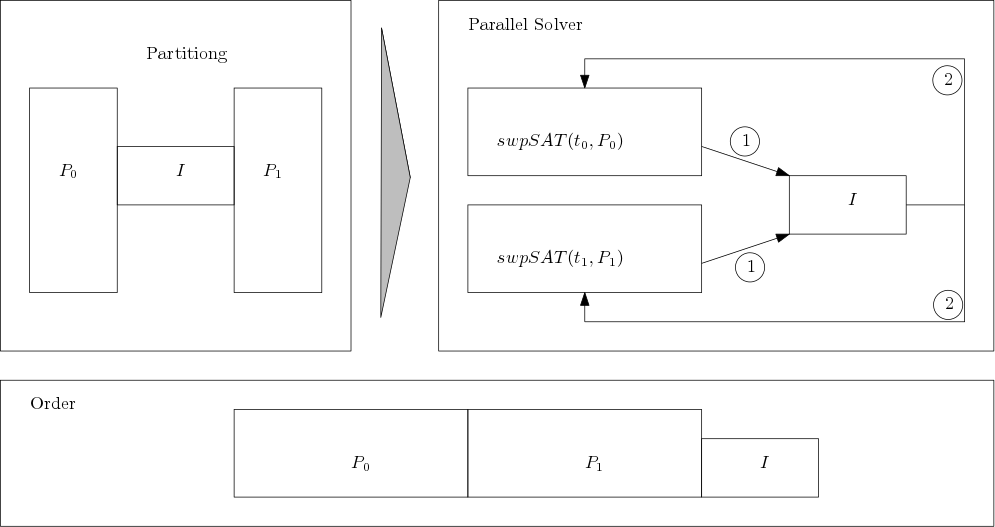
\includegraphics[scale = 0.3]{1/a2.png}
  \end{center}
  \label{a2}
  \end{figure}
We did an experiment to test the performance of this approach. It shows, however a worse performance compared to the original \emph{swpSAT} especially in the aspect of the number of solved problems. It can solve only trivial small problems. According to our observation in the implementation, we think the possible reason is the following: Its sequential version is precisely our swpSAT solver with priorities of unsatisfied clauses. Instead of choosing an unsatisfied clause in whole formula, this approach solves first $P_0$ and then $P_1$ (or inverse) and at last the Intersection $I$. So there is no reason $f$ an improved performance in this parallel search. Worsely, because the priority of the clauses in search, the flip works are done in slave threads are destroyed easily in solving the intersection part, even we take the breaks score in partitioning sets in the count. There are more local minimums are visited in the search path. These  ``traps'', which can be avoided before by an independent chosen clause with variables in another partitioning set, make the search much slower.
\subsection{3nd Approach: Assignment combination}
In consideration of the failure in approach above, in this approach we make the slave threads solve intersection part besides a partition set. First, each slave thread finds a satisfying sub-assignment for the corresponding partitioning set and also the intersection part. Not like the approach 2, here two slave threads may have some different assignments to variables in the boundary of the partitioning. Then the master threads may deal with these differences. That is, we combine these two sub-assignment such that we can get a satisfying assignment or an assignment with only a few conflicts. Then the slave threads will adjust this assignment by make flips in the part of their charge (including the intersection part). 
\begin{figure}[H]
\begin{center}
  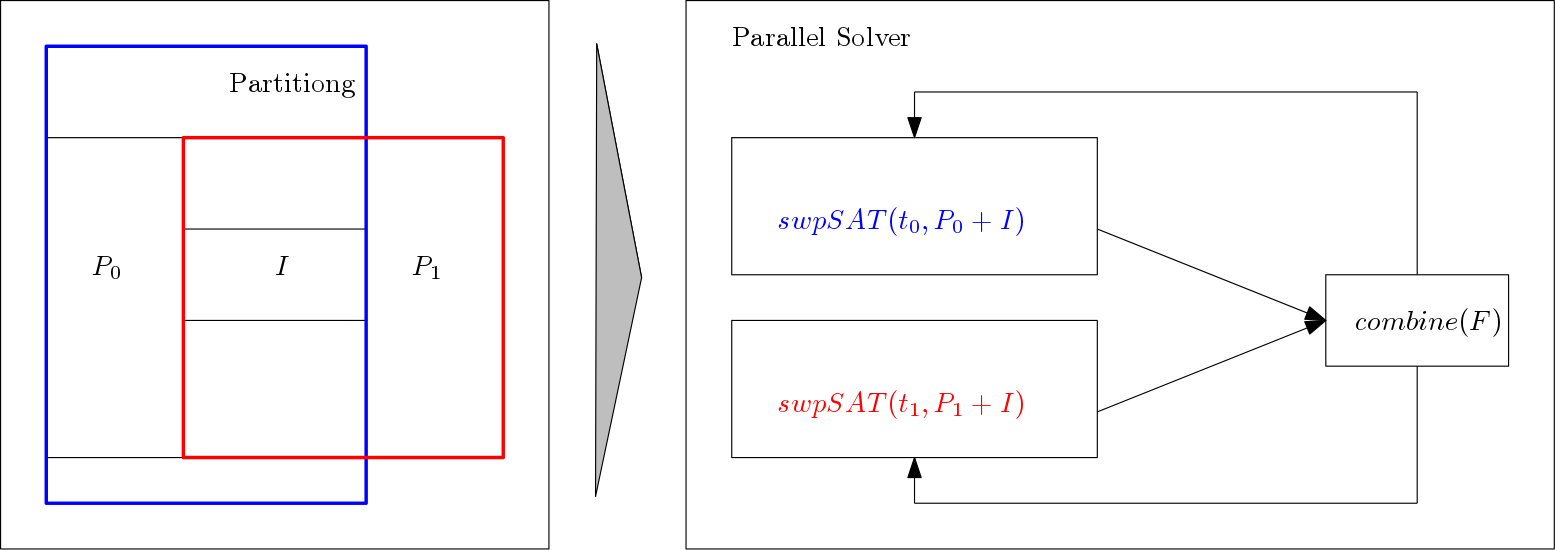
\includegraphics[scale = 0.3]{1/a3.png}
  \end{center}
  \label{a2}
  \end{figure}
For the combination of two sub-assignments, if the assignments of one variable are different in  sub-solutions, there are several cases:\\ 
\\
1. This variable is not the critical one for at least one sub-assignment, so we can assign it as the value in the other sub-assignment.\\
\\
2. If the variable in consideration is critical in both sub-assignment, there are some different policies. The simple one is to assign the variable randomly. We call this policy further $randomCombine$. Another one is to assign the variable as the value suggested by its charging thread. In another word, we combine the assignment according to the partitioning. This policy will not break any clauses in partition set. The slave thread will deal with conflicts in intersection individually in the next round. This policy refers as $partition-based Combine$.\\
\\ In experiment, we compare these two policies. Both policies can not bring a better performance compared with our $swpSAT$ solver. The possible reason is: According to the process in slaver threads, the subassignments  tend to make the variables in other partitioning set the critical ones. Because flipping of these varibales have lower breaks values. In the process of assignment combination, the efforts made in threads are destroyed.  The $partition-based Combine$ process suffers from repeated flips. Even the $randomCombine$ takes more time than the  $swpSAT$ solver to get a solution.
\subsection{4th Approach: Initialization with a guide of formula partitioning}
After the analysis of the failures in the 2 approaches above, we came up with this approach, in which the formula partition information is only used to get an initial solution, and the further search in the whole problem is like our pure portfolio approach. This approach intends to use the partitioning information to get a good initial solution.  A local search from this initial solution with only a few conflicts in the intersections can reduce the search space and prevent long-term cycling in the search. The statistic information shared between the agents encourage the further search the flipping of non critical variables in clauses. \\
\\
\begin{algorithm}[H]
\SetKwInOut{Input}{input}
\SetKwInOut{Output}{output}
\SetKwInOut{Parameter}{parameter}
 \Input{A CNF Formula $F$, number of Processors $n_p$ }
 \Parameter{$Timeout$}
 \Output{a satisfying assignment $A$}
  $sat_0 \leftarrow false$\;
  $sat_1 \leftarrow false$\;
  $sat \leftarrow false$\;
  $A \leftarrow initAssign(F)$\;
 \ForEach{$(Processor_t$ for $t \in \{1, .., n_p\})$}{
    $A_t \leftarrow A$\;
     $i\leftarrow t\%2$\;
 \While {$(!sat_i$  $ \land$ !Timeout$)$}{
	swpSAT($P_i$)\;
	 $sat_i \leftarrow true$\;
	 $A[j] \leftarrow A_i[j]$ for $v_j \in P_i$\;
}
 \While {$(!sat_{1-i}$  $ \land$ !Timeout$)$}{
	 swpSAT($P_{1-i}$)\;
	 $sat_{1-i} \leftarrow true$\;
	 $A[j] \leftarrow A_i{1-i}[j]$ for $v_j \in P_{1-i}$\;
 }
 $A_i \leftarrow A$\;
 \While {$(!sat$  $ \land$ !Timeout$)$}{
 	 swpSAT($F$)\;
 	 $sat\leftarrow true$\;
 	  $A \leftarrow A_i$\;
 }
 }
 \caption{Focused Local Search}
\end{algorithm}  



\clearpage
\section{Evaluation} 
\label{sec:eva}
 %TODO some server information
\subsection{DIMACS standard format}  
All the benchmark formula used in experiments are encoded in the DIMACS standard format\cite{balyo2017proceedings}. This format is the standard format of benchmarks used in SAT competitions. A DIMACS file contains the description of an instance using three types of lines:\\
\\ 1. Comment line: Comment lines give information about the formula for human readers, like the author of the file or the seed used in problem generation. A comment line starts with a lower-case character $c$ and will be ignored by programs:\\ \centerline{\textbf{c} \emph{ this is an example of the comment line }}\\ \\ 2. Problem line: The problem line appears exactly once in each DIMACS format file. The problem line is signified by a lower-case character $p$.  For a formula with $nV$ variables and $nC$ clauses ,the problem line in its DIMACS file is:\\ \centerline{\textbf{p} cnf $nV$ $nC$}\\ \\ 3. Clause descriptor: An clause $\{v_1, v_2,, v_n\}$ in the formula is described in an clause Descriptor:\\ \centerline{\textbf{e} $v_1\; v_2\;  \;v_n$}\\  
\\
Here is the DIMACS format of the formula $F = (v_1 \lor \bar{v_3}) \land (v_2 \lor v_1 \lor \bar{v_1})$:
\begin{center}
\begin{tabular}{l}
c simple F.cnf\\
p cnf 3 2\\
1 -3 0\\
2 3 -1 0 \\
\end{tabular}
\end{center}

\subsection{Benchmarks}
\label{benchmark}
The benchmark instances used in experiments are the 180 uniform instances ( \emph{UNIF}) in random benchmark categories in SAT competition 2017\cite{balyo2017proceedings}. In an  \emph{UNIF} problem file, all the clause have the same length.\\
To generate an instance with $n$ variables and $m$ clauses, the Uniform generation will work in the following way: to construct one clause, $k$ literals are randomly chosen from the $2n$ possible literals. If the generated clause contains multiple copies of the same variables, it will be abandoned. The process generates clauses until m permitted clauses are gathered.\\
In the name of an \emph{UNIF} file, the suffix $k$  denotes the length of clauses. The $r$ indicates the clause-to-variable ratio. The $c$ and $v$ are for the number of clauses and variables, while $s$ is for the seed used in the generation process.
Without flitering, there are at least $60$ ( $33\%$ ) problems form our $180$ benchmark collections are unsatisfiable.
\subsection{Used plots and tables}
the results of the following experiments are all shown in comparision tables and  illusatrated in cactus plots.  \\
\\
\emph{\textbf{Comparison Table}}\\
See Table \ref{tab:com} for example.\\
A comparison table shows the different results of algorithms. The first column contains the
clause length $k$. The  \emph{UNIF} benchmark has $3$ different sizes: $3$SAT, $5$SAT, and $7$SAT. For a $k$SAT instance, each clause contains $k$ variables. The fields of a comparison table in the following columns corresponds to a penalized runtime for the whole $k$SAT set, which assigns a runtime of two times the time limit for an unsolved instance. Because the  \emph{UNIF} benchmark problems without filtering contain a part of unsatisfied problems, we assign penalized time only to problems which can not be solved by any solvers in our whole experiments. There are 61 $3$SAT instances, 89 $5$SAT instances and 66 $7$SAT instances found satisfied in our experiments. Besides the runtime score, the number of solved problems are shown below. The best results in comparison are in bold.
\\
\\
\emph{\textbf{Cactus Plot}}\\
See Figure \ref{Experiment cactus} for an example.\\
A cactus plot shows the performance of different algorithms. The y-axis shows the time in second used to solve the benchmark graphs.  The x-axis is for the number of solved problems by a certain time. Each algorithm corresponds to a curve in different colors. The point $(u, v)$ on a curve means by $v$ seconds the corresponding algorithm have solved  $u$ problems.  \\

\subsection{Random seeds used in Experiments}
\label{sec:seed}
To make our experiments results reproducible and robust, we repeat our tests with three specific seeds. We produce the seeds in experiments as follows: First, we use the sum of characters of the name of the solver to seed the pseudo-random generator in c++.  Then we use this reinitialized generator to produce three random values, which are the seeds used later in our experiments. 
\begin{table}[h!]
%\begin{minipage}{\textwidth}                                                                                         
\begin{center}
    \begin{tabular}{|l|l|l|l|l|p{1cm}|}
\hline 
    solver&name&1.seed&2.seed&3.seed \\ \hline
	\emph{probSAT}&probsat&1988822874&338954226 &858910419 \\ \hline
	yalSAT &yalsat&1851831967&280788293&1956345180 \\ \hline
	our local solver & local&1962042455&1112841915&566263966 \\ \hline
	our parallel solver & parallel &1749729997& 68910537& 473644167 \\ \hline
	
\end{tabular}
\caption[probSAT]{Parameter setting for our solvers and competitors}
\end{center}
%\end{minipage}
\end{table} 
\subsubsection{Soft- and Hardware}
The single-threaded experiments were run on computers that had Two Intel Xeon E5-2683 v4 processors  (2.1 GHz 2x16-cores + 2x16-HT cores) and 512GB RAM. The machine ran the 64-bit version
of  Ubuntu 14.04.5 LTS. The multi-threaded experiments were run on a computer that had Two Intel Xeon E5-2650 v2 processors (16 cores + 16 HT cores) with 128GB DDR3 RAM. The machine ran the 64-bit version of Ubuntu Devel. 
\clearpage
\subsection{Parameter Settings in Experiment}
The $TimeOut$ is set to 5 Minutes in the experiments of local searches.  For the \emph{probSAT} selection heuristic, our local search uses the values for $c_b$ and $\epsilon$ suggested in the \emph{probSAT} paper.  The parameter $\alpha$ and the $tolerence$ $ \tau$ in variances with simulated annealing are generated with the help of the algorithm parameter optimization tool SMAC [29] (sequential model-based algorithm configuration). SMAC ran our algorithms on LARGE problems in the \emph{UNIF} category in SAT 2012 ($75\%$ of the instances training instances,  $25\%$ as test instances) with values $\in [0, 10]$ with step $0.5$ and randomly generated seeds\footnote{Because of high time consume in parameter optimation, we solely compare $\tau$  as a natural number form One to Ten.}.
   \begin{table}[H]
%\begin{minipage}{\textwidth}                                                                                         
\begin{center}
    \begin{tabular}{|l|l|l|l||l|l|l|l|p{1cm}|}
\hline 

    k &\emph{WALK}&\emph{WALK-Local}&\emph{WALK-Global}&\emph{Average}&\emph{Average-Local}&\emph{Average-Global} \\ \hline
    3 & 1& 1 & 10 &  1 & 2& 0.5       \\ \hline  
    5 & 0.5& 1 & 1&  1 & 2& 2 \\ \hline  
    7 & 1& 0.5 & 2&  1 & 2& 0.5  \\ \hline  
 \hline  
    k &\emph{RF}&\emph{RF-Local}&\emph{RF-Global}&\emph{swpSAT}&\emph{$\alpha$/$\tau$}&\emph{SA} \\ \hline  
    3 & 1& 0.5 & 0.5&$Average$ & 1 & $-$\\ \hline 
    5 & 0.5& 2& 9.5&$Average$& 2 & $Local$\\ \hline 
    7 & 0.5& 1& 0.5 &$Average$&2 & $Local$\\ \hline 

	
\end{tabular}
\end{center}
%\end{minipage}
\end{table}
\subsection{Benchmark Generation}
To combine the formula partitioning and SAT local solver, we try to get a relatively balanced partition with small intersection for the hypergraphgraph representation of benchmark SAT problems.  On  \emph{UNIF} benchmark, we try to get graph partitioning using some partitioning algorithms (KaHypar and hmetis). Since the uniform random generation of this benchmark, these problems are without a real-world-like structure. Even with a high imbalance like $0.3$ and high tolerance of intersection size ($50\%$ of edge sizes), the partitioning algorithms take more time than our SAT solver for more than half of our  \emph{UNIF} benchmarks.  To investigate the local search on graphs with proper partitioning, we generate our benchmark COMBINE  using the  \emph{UNIF} benchmark instances.  As the name \emph{COMBINE} suggested, we combine two \emph{UNIF} benchmark instances in one SAT problem and make for the new generated problem with two disjoint subproblems an intersection.  To create a satisfiable formula, we build the intersection based on a pair of random chosen satisfying assignments of the two \emph{UNIF} problems in combination. To get satisfying assignments of  \emph{UNIF} benchmarks, we run different solvers in SAT competitions including \emph{CSCCSAT}, \emph{DCCASAT}, \emph{score2SAT}, \emph{probSAT}, and \emph{yalSAT}. We do not use our local search to collect satisfying assignments. Otherwise, it is possible that after solve the two partitioning sets individually using our local solver, the current assignment is the same or a similar one used for the intersection generation.\\
We combine the \emph{UNIF} problems in consideration of real-world uses. 
We combine 4  pairs of instances in  $3$SAT, $5$SAT problems $7$SAT problems. Besides that, we consider five combinations between  3SAT and 5 SAT instances and three combination of $5$SAT and $7$SAT instances. 
We combine problem in similar vertices size, which corresponds to balanced partitioning in the structure. We also combine one massive problem with a small instance of an imbalanced partitioning. For the intersection generation part, we generate clauses with three vertices in different partitioning sets. \\
We first choose vertices of two partition sets for intersection generation randomly. Here we consider also the balanced intersection and imbalanced intersection. In a balanced intersection, same proportion of vertices in both partitioning sets are chosen to generate the intersection. In an imbalanced intersection, the portions are not the same.  To control the size of the intersection, we also count the number of the clauses in an intersection, if the proposition of the intersection clauses in the clauses number in whole combined problems is upper a specified limit, the generation of intersection is stopped.
\begin{table}[H]
\label{tab:combine big} 
%\begin{minipage}{\textwidth}                                                                                         
\begin{center}
    \begin{tabular}{|l|l|p{1cm}|}
\hline 
Problem &Intersection \\ \hline
k3-r3.94.cnf-k3-r4.04.cnf-0.1-0.1-0.1.cnfP&	1.04\%\\  \hline
k3-r3.96.cnf-k3-r4.06.cnf-0.1-0.1-0.2.cnfP&	1.00\%\\  \hline
k3-r3.98.cnf-k3-r4.0.cnf-0.1-0.1-0.4.cnfP&	1.03\%\\  \hline
k7-r55.0.cnf-k7-r56.0.cnf-0.1-0.2-0.2.cnfP&	15.53\%\\  \hline
k7-r55.0.cnf-k7-r56.0.cnf-0.1-0.4-0.1.cnfP&	6.84\%\\  \hline
k7-r55.0.cnf-k7-r56.0.cnf-0.2-0.2-0.2.cnfP&	12.04\%\\  \hline
k7-r55.0.cnf-k7-r56.0.cnf-0.2-0.4-0.1.cnfP&	7.53\%\\  \hline
k7-r55.0.cnf-k7-r56.0.cnf-0.4-0.1-0.4.cnfP&	6.38\%\\  \hline
k7-r55.0.cnf-k7-r56.0.cnf-0.4-0.2-0.1.cnfP&	7.35\%\\  \hline
k7-r55.0.cnf-k7-r56.0.cnf-0.4-0.4-0.2.cnfP&	6.11\%\\  \hline
k7-r57.0.cnf-k7-r60.0.cnf-0.1-0.1-0.2.cnfP&	16.67\%\\  \hline
k7-r57.0.cnf-k7-r60.0.cnf-0.1-0.1-0.4.cnfP&	25.21\%\\  \hline
k7-r57.0.cnf-k7-r60.0.cnf-0.1-0.2-0.2.cnfP&	14.77\%\\  \hline
k7-r57.0.cnf-k7-r60.0.cnf-0.1-0.4-0.1.cnfP&	6.46\%\\  \hline
k7-r57.0.cnf-k7-r60.0.cnf-0.2-0.1-0.2.cnfP&	13.92\%\\  \hline
k7-r57.0.cnf-k7-r60.0.cnf-0.2-0.2-0.4.cnfP&	11.40\%\\  \hline
k7-r57.0.cnf-k7-r60.0.cnf-0.2-0.4-0.2.cnfP&	7.08\%\\  \hline
k7-r57.0.cnf-k7-r60.0.cnf-0.4-0.1-0.4.cnfP&	5.88\%\\  \hline
k7-r57.0.cnf-k7-r60.0.cnf-0.4-0.2-0.4.cnfP&	6.86\%\\  \hline
k7-r57.0.cnf-k7-r60.0.cnf-0.4-0.4-0.4.cnfP&	5.81\%\\  \hline
k7-r58.0.cnf-k7-r62.0.cnf-0.1-0.1-0.1.cnfP&	9.09\%\\  \hline
k7-r58.0.cnf-k7-r62.0.cnf-0.1-0.1-0.2.cnfP&	16.67\%\\  \hline
k7-r58.0.cnf-k7-r62.0.cnf-0.1-0.1-0.4.cnfP&	25.07\%\\  \hline
k7-r58.0.cnf-k7-r62.0.cnf-0.1-0.2-0.1.cnfP&	9.09\%\\  \hline
k7-r58.0.cnf-k7-r62.0.cnf-0.1-0.2-0.4.cnfP&	14.68\%\\  \hline
k7-r58.0.cnf-k7-r62.0.cnf-0.1-0.4-0.4.cnfP&	6.36\%\\  \hline
k7-r58.0.cnf-k7-r62.0.cnf-0.2-0.1-0.1.cnfP&	9.09\%\\  \hline
k7-r58.0.cnf-k7-r62.0.cnf-0.2-0.1-0.2.cnfP&	13.96\%\\  \hline
k7-r58.0.cnf-k7-r62.0.cnf-0.2-0.2-0.2.cnfP&	11.58\%\\  \hline
k7-r58.0.cnf-k7-r62.0.cnf-0.2-0.4-0.2.cnfP&	6.97\%\\  \hline
k7-r58.0.cnf-k7-r62.0.cnf-0.4-0.1-0.4.cnfP&	5.98\%\\  \hline
k7-r58.0.cnf-k7-r62.0.cnf-0.4-0.4-0.4.cnfP&	5.60\%\\  \hline
k7-r59.0.cnf-k7-r87.79-v90.cnf-0.1-0.1-0.4.cnfP&	1.30\%\\  \hline
k7-r59.0.cnf-k7-r87.79-v90.cnf-0.1-0.2-0.2.cnfP&	2.52\%\\  \hline
k7-r59.0.cnf-k7-r87.79-v90.cnf-0.1-0.4-0.2.cnfP&	4.88\%\\  \hline
\end{tabular}
 \caption[Caption for LOF]{COMBINE problems with small intersection ($\frac{numCI}{numC} > 1\%$)\footnotemark}
\end{center}
%\end{minipage}
\end{table} 
\footnotetext{numCI: number of clauses in intersetcion}

\begin{table}[H]
\label{tab:combine small} 
%\begin{minipage}{\textwidth}                                                                                         
\begin{center}
    \begin{tabular}{|l|l|p{1cm}|}
\hline 
Problem &Intersection \\ \hline
k3-r3.92.cnf-k3-r3.88.cnf-0.2-0.1-0.4.cnfP&	0.38\%	\\   \hline
 k3-r3.92.cnf-k3-r3.88.cnf-0.2-0.4-0.1.cnfP&	0.13\%	\\   \hline
 k3-r3.94.cnf-k3-r4.04.cnf-0.1-0.2-0.1.cnfP&	0.36\%	\\   \hline
 k3-r3.94.cnf-k3-r4.04.cnf-0.1-0.4-0.4.cnfP&	0.11\%	\\   \hline
 k3-r3.94.cnf-k3-r4.04.cnf-0.2-0.1-0.2.cnfP&	0.37\%	\\   \hline
 k3-r3.94.cnf-k3-r4.04.cnf-0.2-0.2-0.1.cnfP&	0.27\%	\\   \hline
 k3-r3.94.cnf-k3-r4.04.cnf-0.4-0.2-0.4.cnfP&	0.11\%	\\   \hline
 k3-r3.94.cnf-k3-r4.04.cnf-0.4-0.4-0.4.cnfP&	0.09\%	\\   \hline
 k3-r3.96.cnf-k3-r4.06.cnf-0.1-0.2-0.2.cnfP&	0.37\%	\\   \hline
 k3-r3.96.cnf-k3-r4.06.cnf-0.1-0.4-0.1.cnfP&	0.11\%	\\   \hline
 k3-r3.96.cnf-k3-r4.06.cnf-0.2-0.1-0.2.cnfP&	0.35\%	\\   \hline
 k3-r3.96.cnf-k3-r4.06.cnf-0.2-0.2-0.2.cnfP&	0.27\%	\\   \hline
 k3-r3.96.cnf-k3-r4.06.cnf-0.2-0.4-0.2.cnfP&	0.13\%	\\   \hline
 k3-r3.96.cnf-k3-r4.06.cnf-0.4-0.1-0.2.cnfP&	0.10\%	\\   \hline
 k3-r3.96.cnf-k3-r4.06.cnf-0.8-0.8-0.05.cnfP&	0.06\%	\\   \hline
 k3-r3.98.cnf-k3-r4.0.cnf-0.1-0.2-0.1.cnfP&	0.38\%	\\   \hline
 k3-r4.267-v11000.cnf-k5-r16.2.cnf-0.8-0.8-0.05.cnfP&	0.52\%	\\   \hline
 k3-r4.267-v11200.cnf-k5-r16.8.cnf-0.8-0.8-0.05.cnfP&	0.49\%	\\   \hline
 k3-r4.267-v11600.cnf-k5-r17.0.cnf-0.8-0.8-0.05.cnfP&	0.52\%	\\   \hline
 k3-r4.267-v7400.cnf-k5-r17.2.cnf-0.8-0.8-0.05.cnfP&	0.34\%	\\   \hline
 k3-r4.267-v9600.cnf-k5-r17.4.cnf-0.8-0.8-0.05.cnfP&	0.42\%	\\   \hline
 k5-r21.117-v200.cnf-k5-r16.0.cnf-0.1-0.1-0.2.cnfP&	0.04\%	\\   \hline
 k5-r21.117-v200.cnf-k5-r16.0.cnf-0.2-0.1-0.2.cnfP&	0.09\%	\\   \hline
 k5-r21.117-v200.cnf-k5-r16.0.cnf-0.4-0.1-0.4.cnfP&	0.17\%	\\   \hline
 k5-r21.117-v220.cnf-k5-r17.6.cnf-0.8-0.8-0.05.cnfP&	0.01\%	\\   \hline
 k5-r21.117-v280.cnf-k5-r16.4.cnf-0.1-0.1-0.4.cnfP&	0.06\%	\\   \hline
 k5-r21.117-v280.cnf-k5-r16.4.cnf-0.2-0.1-0.1.cnfP&	0.12\%	\\   \hline
 k5-r21.117-v280.cnf-k5-r16.4.cnf-0.4-0.1-0.1.cnfP&	0.23\%	\\   \hline
 k5-r21.117-v290.cnf-k5-r16.6.cnf-0.1-0.1-0.2.cnfP&	0.06\%	\\   \hline
 k5-r21.117-v290.cnf-k5-r16.6.cnf-0.2-0.1-0.4.cnfP&	0.12\%	\\   \hline
 k5-r21.117-v290.cnf-k5-r16.6.cnf-0.4-0.1-0.1.cnfP&	0.24\%	\\   \hline
 k7-r59.0.cnf-k7-r87.79-v90.cnf-0.2-0.1-0.4.cnfP&	0.21\%	\\   \hline
 k7-r59.0.cnf-k7-r87.79-v90.cnf-0.2-0.2-0.4.cnfP&	0.41\%	\\   \hline
 k7-r59.0.cnf-k7-r87.79-v90.cnf-0.2-0.4-0.2.cnfP&	0.80\%	\\   \hline
 k7-r59.0.cnf-k7-r87.79-v90.cnf-0.4-0.1-0.4.cnfP&	0.04\%	\\   \hline
 k7-r59.0.cnf-k7-r87.79-v90.cnf-0.4-0.2-0.4.cnfP&	0.09\%	\\   \hline
 k7-r59.0.cnf-k7-r87.79-v90.cnf-0.4-0.4-0.2.cnfP&	0.18\%	\\   \hline
 k7-r87.79-v102.cnf-k5-r17.8.cnf-0.8-0.8-0.05.cnfP&	0.00\%	\\   \hline
 k7-r87.79-v106.cnf-k5-r18.0.cnf-0.8-0.8-0.05.cnfP&	0.01\%	\\   \hline
 k7-r87.79-v110.cnf-k5-r18.2.cnf-0.8-0.8-0.05.cnfP&	0.01\%	\\   \hline

\end{tabular}
\caption{COMBINE problems with small intersection ($\frac{numCI}{numC} < 1\%$)}
\end{center}
%\end{minipage}
\end{table} 

\subsection{Experiments}
\subsubsection{Experiment 1: initAssign(F)}
\label{sec:Experiment 1}
Experiment 1 compares three strategies of initialization in our solver. In the original $pobSAT$ algorithm, the first step $randomInit$  builds a complete assignment randomly in the initialization phase. \\ \\The $biasInit$ suggestion is assign variables based on occurrences of their literals. It assigns \emph{true} to variables whose positive literal occurs more than its negative literal.The number of unsatisfied clauses in the bias initialized assignment of a kSAT problem is limited to $\frac{numC}{2^k}$. Our hyperthesis in the assignment initialization is that an initial solution with good quality can speed up the search generally. \\ \\ In a combination of these two variants, the $randomBiasInit$, the boolean value is assigned to variables based on bias randomly on literals occurrences. The probability to assign true to variable $v_i$ is $\frac{posOccurences[i]}{posOccurences[i]+negOccurences[i]}$. As a stochastic bias initialization, it can get an assignment with expectedly few unsatisfied clauses. With the robustness of a random process, the $randomBiasInit$ permit local stucks. \\\\ In a local search algorithm, it is normal that a replacement of the current solution by a new initial solution after a limit of the number of tries. However, in our implementation, the current assignment will be changed locally with flippings of variables after the initialization. In the following table, we compare three variants in the original \emph{probSAT} algorithms. Based on the results of this experiments, we will determine the way of initialization in our heuristic solver for the problems with different length. 
\\
\begin{table}[H]
\label{tab:com}
%\begin{minipage}{\textwidth}                                                                                         
\begin{center}
    \begin{tabular}{|l|l|l|l|p{1cm}|}
\hline 
    k &$RandomInit$&$BiasInit$&$Bias$-$RandomInit$ \\ \hline
	3&9221.9 &9157.76 &\textbf{9078.27} \\ 
	&\textbf{55} &54 & \textbf{55} \\ \hline
	5&7143.9&\textbf{4351.09}&4582.54\\ 
	&82 &\textbf{87} &\textbf{87}\\ \hline
	7&6238.51&\textbf{5421.9}& 6310.7\\
	&60 & 60 & 60 \\ \hline
	
\end{tabular}
\caption{For 3SAT problems, the initializations get similar performances. According to the PAR2-score of the benchmark sets, the two bias initiliazatios show improvment with about $60\%$ percentage reduction in penalized runtime for 5SAT problems.  the \emph{BiasInit} shows its Efficiency in 7SAT problems. The search is about $14\%$ faster than the original \emph{probSAT} algorithm with a (bias) randomly generated initilization. }
\end{center}
%\end{minipage}
\end{table} 
\clearpage
\begin{figure}[H]
 \label{Experiment cactus}
  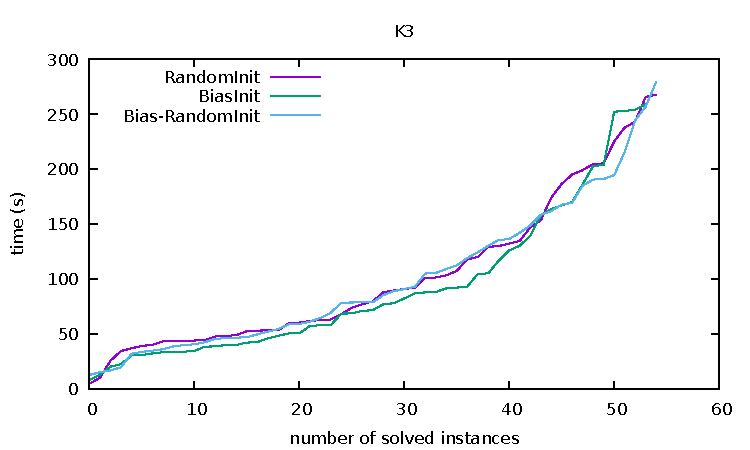
\includegraphics[scale =0.8]{DATA/K3/e1.pdf}
  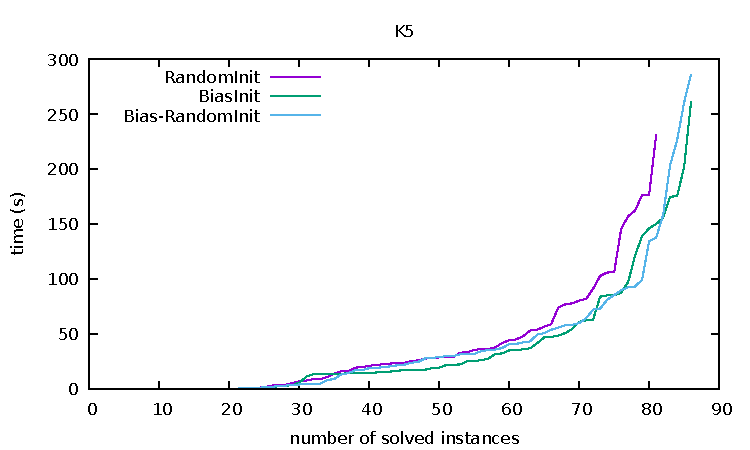
\includegraphics[scale = 0.8]{DATA/K5/e1.pdf}
  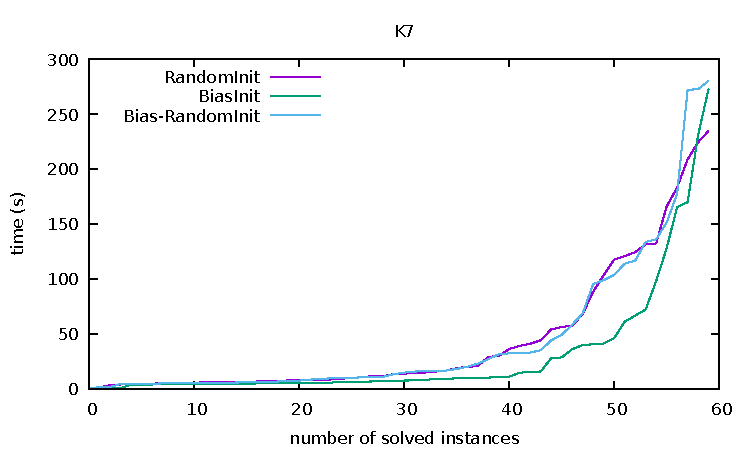
\includegraphics[scale = 0.8]{DATA/K7/e1.pdf}
  \label{Experiment 1 k357 cactus plot}
  \caption{Three suggestions have very similar performance for 3SAT problems. In our solver, we use $RanomInit$ for 3SAT as initiliazation method because of its simplify. Two bias suggestions show advantages especially for huge 5SAT instances. For 7SAT problems, the two random Initialization are similar in performance, while the bias initialization shows its efficiency.}
\end{figure}
\clearpage
\subsubsection{Experiment 2: pickVar(F)} 
\label{sec:Experiment 2} 
The \emph{probSAT} algorithm paradigm introduced in section make pickVar as a randomized process To pick a variable for flipping in a chosen clause, we need to measure the score of all the literals in the classes and then model the probability distribution of the scores.  In the observation of the implementation, this stochastic process is very time-consuming.  The \emph{probSAT} takes a lot of time in the first phase of the search and also go around with few conflicts in the last steps. However, in the first phase of the search, picking flippings greedy can lead the search quickly to the regions of interest.In our examples in the table \ref{parma}. The probability to ignore the greedy literal is 30\% for the 3SAT example and more than  50\% for 5SAT and 7SAT.  Then in the last steps of the search, where the search can reach the final satisfying assignment by a few deterministic steps, this \emph{probSAT} algorithm may make  ``unintelligent'', decisions with some probability and miss the critical steps. \\
To make the selection more greedily, we use a random walk to choose policy between greedy one and the \emph{probSAT} heuristic.  In our algorithm, we refer the literals with no clause breaking as a greedy literal where greedy literal means the one with least break scores in original \emph{walkSAT}. The greefy literal will be chosen in the greedy heuriscti and also be possible be chosen in \emph{probSAT} heuristic. The intention of giving the literals with zero breaks more probability to be chosen is the observation that the time-consuming \emph{probSAT} may choose the breaking literals with high probability (see Table~\ref{parma}).  To speed up this selection process and increase the randomness of the process, we just picked one greedy literal randomly as the greedy candidate for flipping.  To avoid cycling in one region, we record the status information in the process.  If the flips of chosen greedy literal have not been repeated many times, the selection will prefer another variable with a little breakscore, which has not been flipped so many times.  

\begin{table}[h!]
\label{parma}
\begin{center}
\begin{tabular}{|l|l|l|l|p{3cm}|}\hline 
k&  Breaks &          Probability  \\ \hline     
3&  $\{0, 1, 1\}$ & $\{70\%, 15\%, 15\%\}$   \\ \hline         
5 &  $\{0, 1, 1, 1, 1\}$   & $\{  48\%, 13\%, 13\%, 13\%, 13\%\}$\\ \hline
7 & $\{0, 1, 1, 1, 1, 1, 1\}$&    $\{  47\%, 9\%, 9\%, 9\%, 9\%\}$\\ \hline
\end{tabular}
\caption{In this table, we list three examples in 3SAT , 5SAT and 7SAT problem with probabilitys of the \emph{probSAT}. Here we have in the chosen clause a greedy literal and other literals with breakscore 1.  With the  $\Gamma$  function with the recommended parameters in the original \emph{probSAT} paper, we show in the 3.column the probabilities of each literal for flipping.}
\end{center}
%\end{minipage}
\end{table}  
\begin{table}[h!]
%\begin{minipage}{\textwidth}                                                                                         
\begin{center}
    \begin{tabular}{|l|l|l|l|p{3cm}|}
\hline 
    k &\emph{probSAT}&\emph{WALK}&\emph{Average}&\emph{Random-Flip} \\ \hline
	3&9221.9 (55)&7430.12 (57)&\textbf{6161.11}(\textbf{61})&8362.42 (55) \\ \hline
	5&7143.9 (82)&4433.05 (87)&\textbf{3308.16}(\textbf{89})&4052.47(87)\\ \hline

	7& 	6238.51(\textbf{60})& 6358.76(\textbf{60})&6525.597(59)&\textbf{5800.46}(\textbf{60})\\ \hline
	
\end{tabular}
\caption{With the comparison of three Variant of \emph{pickVar}  with the staochastic selection in \emph{probSAT}, our suggestions are faster and solve more instances in K3 and K5. For 3SAT, our suggestions have better performances. The $WALK$ and $Average$ can solve more problems. The best one is the $Average$ (with $\alpha = 1$), which solves $10\%$ more problems. The $Average$ shows advantages also for 5SAT problems, which can solve $8\%$ more problems than the \emph{probSAT} with only $46\%$ time (in PAR-2 schema). For K7,  there are no noticeable differences in results.}
\end{center}
%\end{minipage}
\end{table} 
\clearpage
\begin{figure}[H]
\begin{center}
  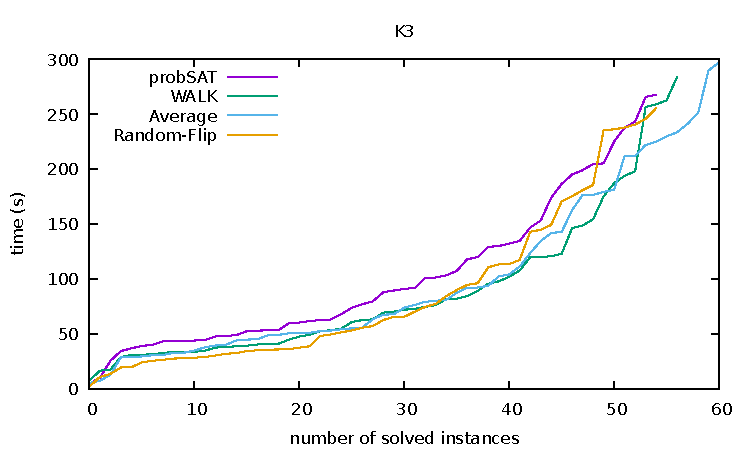
\includegraphics[scale = 0.8]{DATA/K3/e2.pdf}
    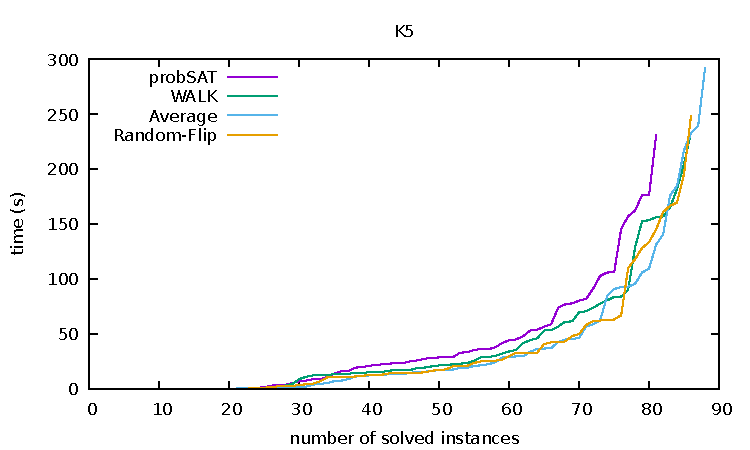
\includegraphics[scale = 0.8]{DATA/K5/e2.pdf}
      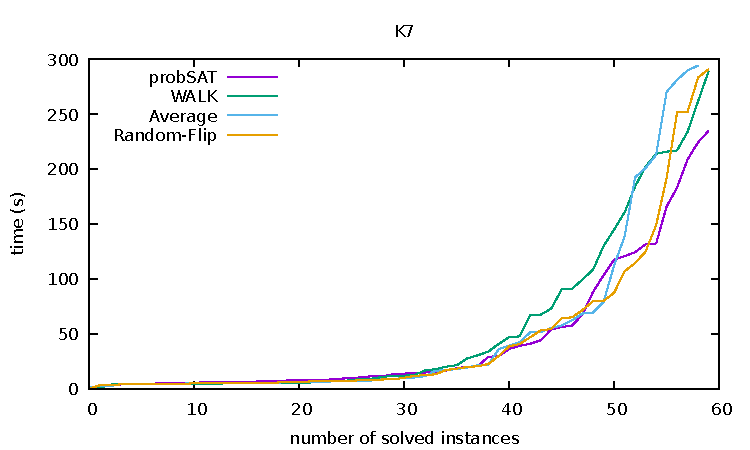
\includegraphics[scale = 0.8]{DATA/K7/e2.pdf}

  \end{center}
  \caption{Our suggestions are faster than the \emph{probSAT} algorithm in 3SAT problems. The \emph{Averrage} shows an absolute improvement except for a few trivial small instances. For 5SAT problems,the improvement through our suggestions are big and stable. They solve more problems efficiently. For 7SAT problems, the \emph{WALK} and \emph{Average} have generally worse inperformance. The \emph{Random-Flip} can solve some number of problems as the original \emph{probSAT} and has shown littel improvement in performance within $125$ Seconds}

  \label{Experiment 2 cactus plot}
  \end{figure}
\clearpage
\subsubsection{Experiment 3: Simulated Annealing} 
\label{sec:Experiment 3}
To use the technique \emph{simulated annealing}, we need measure the quality of the current solution.  One traditional way is to use the number of conflicts. Besides it, we propose the number of greedy literals in the chosen clause. Our hyperthesis behind this idea is that if the current solution is near a satisfying assignment without conflicts,  it is likely to break a clause by a flipping.  And in such case, there should not be only a few greedy literals exist in the chosen clause. Furthermore,  this local quality is more specific about the chosen clause not generally about the whole search progress. \\
\\
With definition of the qualitity $q$, the paramters $\alpha$ is defined as $\alpha = \tau \times (c)^{-q}$. Here the paramter $c$ is in [2, 6]. The noise value $\alpha$ is proportional to the probability of a random walk. With the help of simulated annealing, the search to can measure its current situation. If the quality of the current solution is bad, the search will have a big noise, and thus the search will prefer random literals for flippings. The search can take advantages of random algorithm and can get out of stuck in one regions. That will spped up the search in the first phase. With the improvement of the solution quslity $q$, the search is close to a satisfying assignment. To avoid passing the critical steps, the search will prefer greedy literals. \\
\\
Another thing to mention is that in our implementation we set up a lookup table for the exponential values of the parameter $c_b$ for the repeated calculations of $\Gamma$ function. To reuse exponential values in variants with the simulated annealing, we use the same  $c_b$ as parameter. \\
\\
\begin{table}[H]
%\begin{minipage}{\textwidth}                                                                                         
\begin{center}
    \begin{tabular}{|l|l|l|l|l|l|p{2cm}|}
\hline 

    k &\emph{Average}&\emph{Average-Local}&\emph{Average-Global} &\emph{RF}& \emph{RF-Local}& \emph{RF-Global} \\ \hline      
    3 &$5.43\%$&$2.43\%$&$5.43\%$&$9.98\%$&$10.01\%$&$3.13\%$\\ \hline
    5& $4.07\%$&$0.35\%$&$0.00\%$&$9.18\%$&$9.17\%$&$0.33\%$\\ \hline
    7&$2.28\%$&$0.03\%$&$0.00\%$&$4.30\%$&$4.14\%$&$0.05\%$\\ \hline
\end{tabular}
\end{center}
%\end{minipage}
\caption{To check that the simulated annealing with the parameters in our experiments will change the behavior of the search, we count the number of greedy flips and the number of random flips for the whole problem set. Through our observation, using the parameters we choose, the fraction of greedy flips in total flips are changed. This table shows the values for two variants \emph{Average} and \emph{Random-Flip} for example. }
\end{table} 
Based on the results of experiment 3 (~\ref{sec:Experiment 3}) , we modify our three heuristics with improvement of simulated annealing. We refer the new improved varinats as \emph{Walk.}, \emph{Average.} and \emph{Random-flip.}. In erperiment 4, we list the performances of these variants.\\
\\
In the following, we show our results in our experiments  of  our three variants \emph{WALK}, \emph{Average} and \emph{Random-Flip} with simulated annealing and compare these two definitions of qualities.

\clearpage
\textbf{WALK with Simulated Annealing}\\
\begin{table}[H]
%begin{minipage}{\textwidth}                                                                                         
\begin{center}
    \begin{tabular}{|l|l|l|l|p{3cm}|}
\hline 
    k &\emph{WALK}&\emph{WALK-Local}&\emph{WALK-Global} \\ \hline      
    3 &\textbf{7430.12}(\textbf{57})&	8346.76(56)	&9023.96(56)  \\ \hline
    5&4433.05(87)	&3330.61(89)	&\textbf{3117.45}(\textbf{89}) \\ \hline
    7&6358.76(60)	&\textbf{5409.67}(\textbf{61})&	6566.06(59) \\ \hline	

\end{tabular}
\end{center}
%\end{minipage}
\end{table} 
\begin{figure}[H]
\begin{center}
  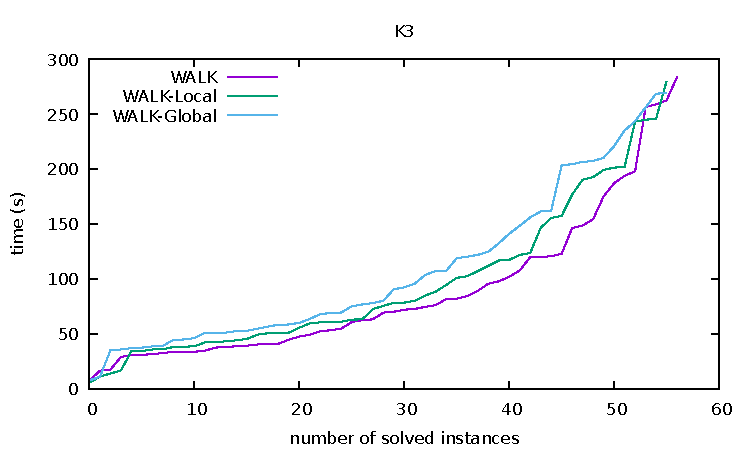
\includegraphics[scale = 0.8]{DATA/K3/e3w.pdf}
  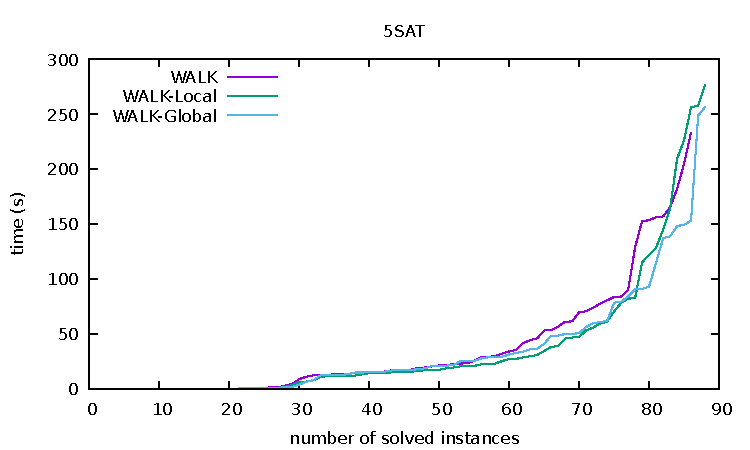
\includegraphics[scale = 0.8]{DATA/K5/e3w.pdf} 
  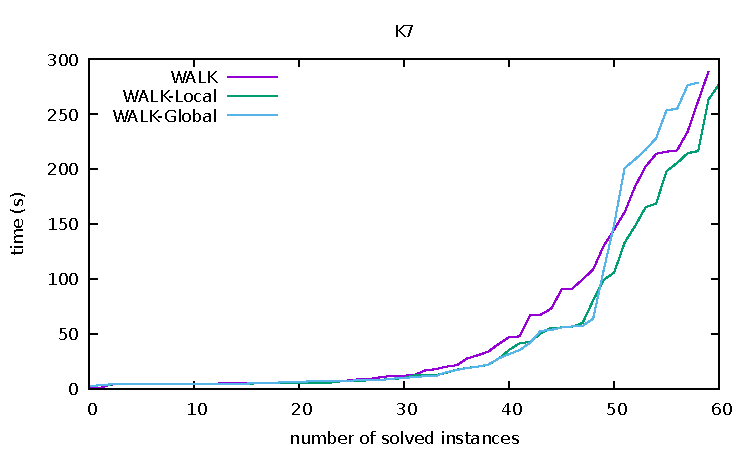
\includegraphics[scale = 0.8]{DATA/K7/e3w.pdf} 
  \caption{For 3SAT, the two combination with simulated Annealing show worse performance than the original \emph{WALK}. The combinations  have also shown their  efficiency in solving huge 5SAT problems. The \emph{Global} shows its advantages for 7SAT problems.
}
  \end{center}
  \label{Experiment 3 WALK cactus plot}
  \end{figure}
  \clearpage
\textbf{ Average with Simulated Annealing}
 \begin{table}[H]
%begin{minipage}{\textwidth}                                                                                         
\begin{center}
    \begin{tabular}{|l|l|l|l|p{3cm}|}
\hline 
   k &\emph{Average}&\emph{Average-Local}&\emph{Average-Global} \\ \hline      
    3 & \textbf{6161.11}(\textbf{61})	&9254.18(53)&	9870.25(53) \\ \hline
    5& 3308.16(89)	&\textbf{2793.32}(89)&	2939.74(89)\\ \hline
    7& 6525.59(59)&\textbf{	3829.95}(\textbf{65})	&5738.2(61)\\ \hline
    \end{tabular}
\end{center}
%\end{minipage}
\end{table}
  \begin{figure}[H]
\begin{center}
  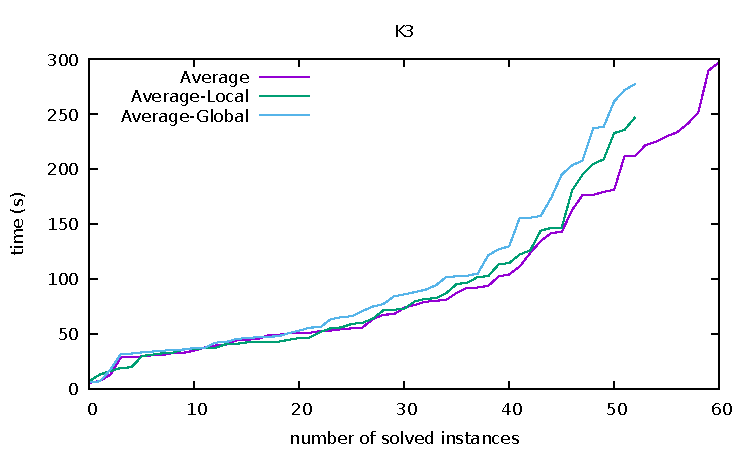
\includegraphics[scale = 0.8]{DATA/K3/e3a.pdf}
    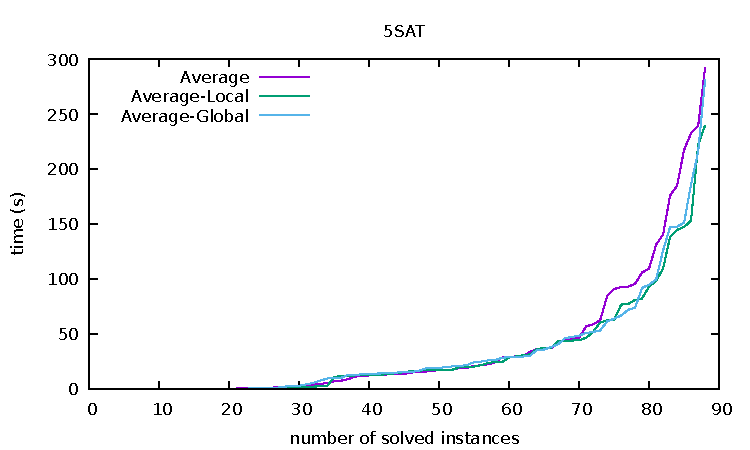
\includegraphics[scale = 0.8]{DATA/K5/e3a.pdf}
      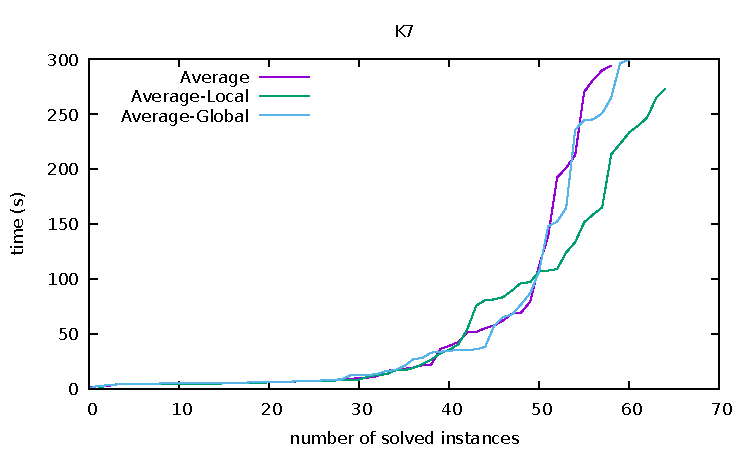
\includegraphics[scale = 0.8]{DATA/K7/e3a.pdf}
  \end{center}
  \caption{ The original \emph{Average} can solve $15\%$ more problems in 3SAT. For 5SAT, there are not noticabel differences in aspect of number of solved problems or the runtime. For 7SAT problems, the \emph{Local} version can solve 6  huge problems more than the original \emph{Average} within less runtime.}
  \label{Experiment 4 k3 cactus plot}
  \end{figure}
 \clearpage
\textbf{Random-Flip with Simulated Annealing} 
  \begin{table}[H]
%\begin{minipage}{\textwidth}                                                                                         
\begin{center}
    \begin{tabular}{|l|l|l|l|p{3cm}|}
\hline 
    k &\emph{Random-Flip}&\emph{Random-Flip-Local}&\emph{Random-Flip-Global} \\ \hline      
    3 &  8362.42(55)&8409.8(55)	&\textbf{7308.01}(\textbf{58})\\ \hline
    5&4052.47(87)&	4132.07(87)&\textbf{4003.06}(\textbf{88}) \\ \hline
    7& 5800.46(60) &6792.23(59) &	\textbf{4903.61}(\textbf{60})\\ \hline	
\end{tabular}
\end{center}
%\end{minipage}
\end{table}
  \begin{figure}[H]
\begin{center}
  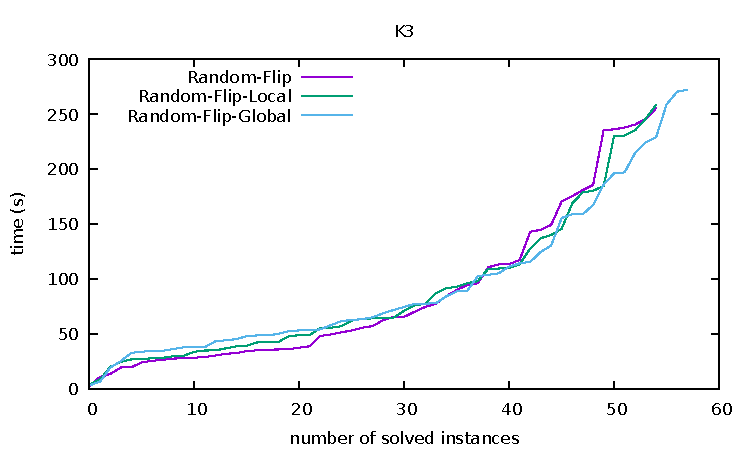
\includegraphics[scale = 0.8]{DATA/K3/e3r.pdf}
  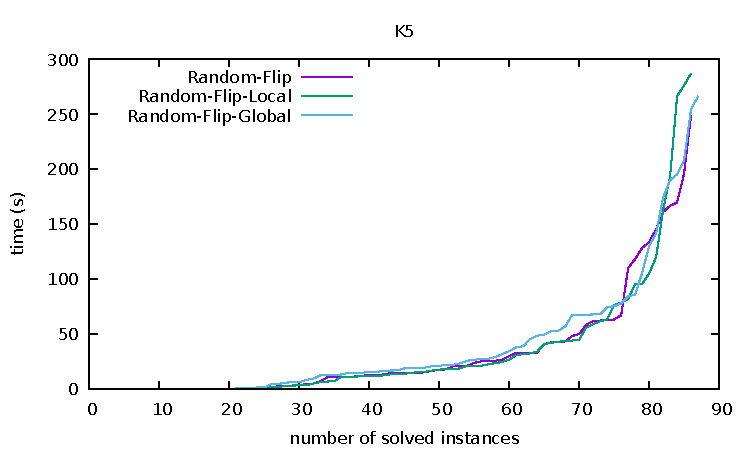
\includegraphics[scale = 0.8]{DATA/K5/e3r.pdf}
    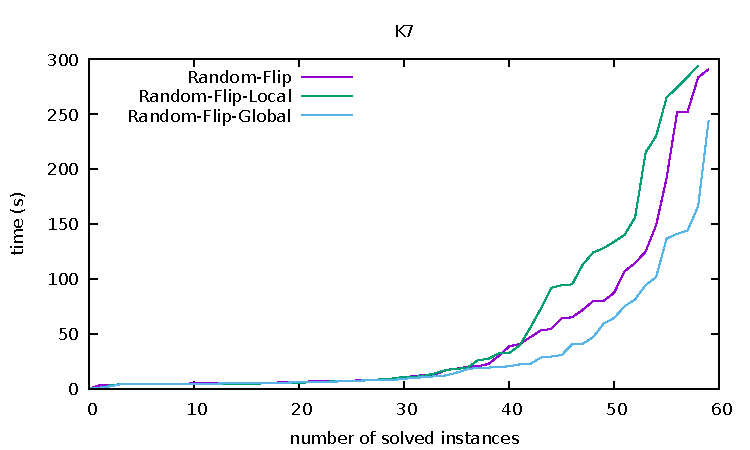
\includegraphics[scale = 0.8]{DATA/K7/e3r.pdf}
    \caption{
The performances of these three algorithms are guiet semiliar for 3SAT and 5SAT problems.  For 7SAT set, the \emph{Local} get worst performance while the variant \emph{Global} has shown  advantages in solving huge problems.}
  \end{center}
  \end{figure}
  \clearpage  
  
\subsubsection{Experiment 4: 2017-UNIF Comparision (local)} 
\label{sec:Experiment 4}
In the table \ref{tab:UNIF}, we list the comparison of our variants with \emph{probSAT} and \emph{yalSAT}. generally, our variants get advantages in runtime and the number of solved problems.
According to the comparison of performances of these three variants,  we set the settings of our final SAT solver \emph{swpSAT} as following: For 3SAT problems, we choose \emph{randINIT} for initilizataion and the \emph{Average}  without simulated annealing as \emph{pickVar} heuristic. For 5SAT and 7SAT problems, we use the \emph{biasINIT} and \emph{Average-Local}.  \\
We count in the search the total number of flips for a problem set. There are no noticeable differences in the average number of flips per second\footnote{Here we consider the solved instances without runtime penalization}. That proves that the improvement we get with our variants is more from the advantages of our algorithms but not the implementation.
   \begin{table}[H]
   \label{tab:UNIF}
%\begin{minipage}{\textwidth}                                                                                         
\begin{center}
    \begin{tabular}{|l|l|l|l|l|p{3cm}|}
\hline 

    k &\emph{probSAT}&\emph{yalSAT}&\emph{WALK}&\emph{Average/swpSAT}&\emph{Random-Flip} \\ \hline      
    3 &9221.9&17062.35&7430.12&\textbf{6161.11} &7308.01\\ 
    &55&41&57&\textbf{61}&58\\ \hline
    5& 7143.9&5676.63&3330.61&\textbf{2939.74}&4003.06\\ 
    &82&85&\textbf{89}&\textbf{89}&88\\ \hline
    7& 6238.51&10063.4&5409.67&\textbf{3829.95}&4903.61\\
    &60&54&61&\textbf{65}&60\\ \hline
	
\end{tabular}
\end{center}
\caption{Comparision in UNIF}
%\end{minipage}
\end{table}
   \begin{table}[H]
   \label{tab:flips}
%\begin{minipage}{\textwidth}                                                                                         
\begin{center}
    \begin{tabular}{|l|l|l|l|l|p{3cm}|}
\hline 

    k &\emph{probSAT}&\emph{WALK}&\emph{Average}/\emph{swpSAT}&\emph{Random-Flip} \\ \hline      
    3& 954426 &946662 &\textbf{1012761}&988477 \\ \hline
    5& 389453&\textbf{443172}&414765&423364\\ \hline
    7& 248025 &237387 &\textbf{248028}&221107 \\ \hline
	
\end{tabular}
\end{center}
\caption{Average flips per second}
%\end{minipage}
\end{table}
  \begin{figure}[H]
\begin{center}
  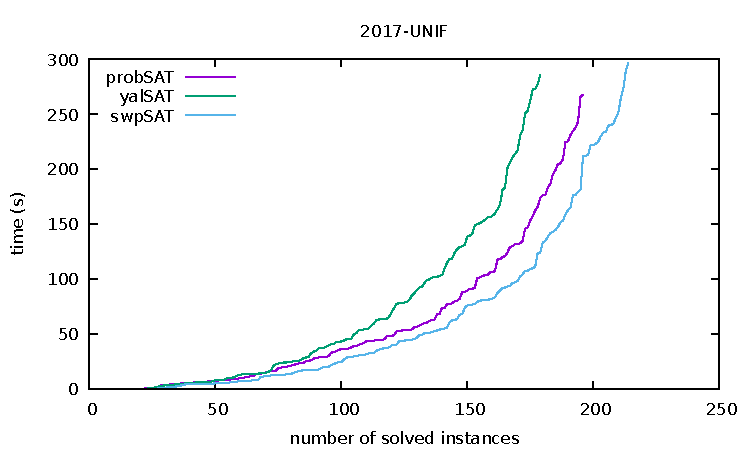
\includegraphics[scale = 1]{DATA/UNIF/e5.pdf}
  \end{center}
  \caption{swpSAT get best performance in UNIF comparing to \emph{probSAT} and \emph{yalSAT} }
  \label{Experiment 9 all cactus plot}
  \end{figure} 
\clearpage
\clearpage
  \begin{figure}[H]
\begin{center}
  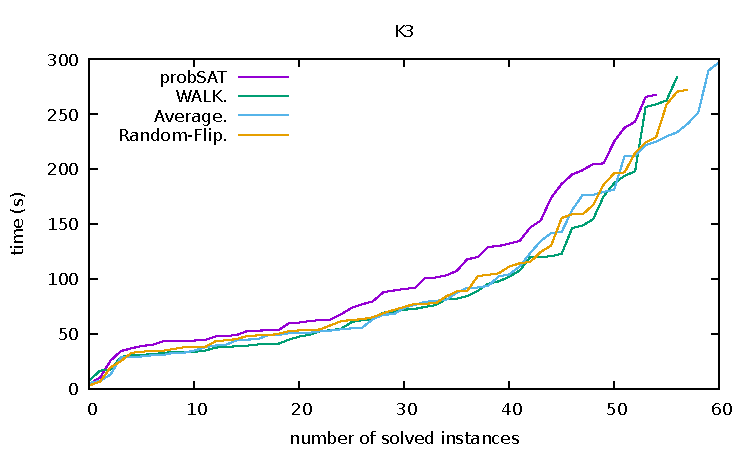
\includegraphics[scale = 0.8]{DATA/K3/e4.pdf}
    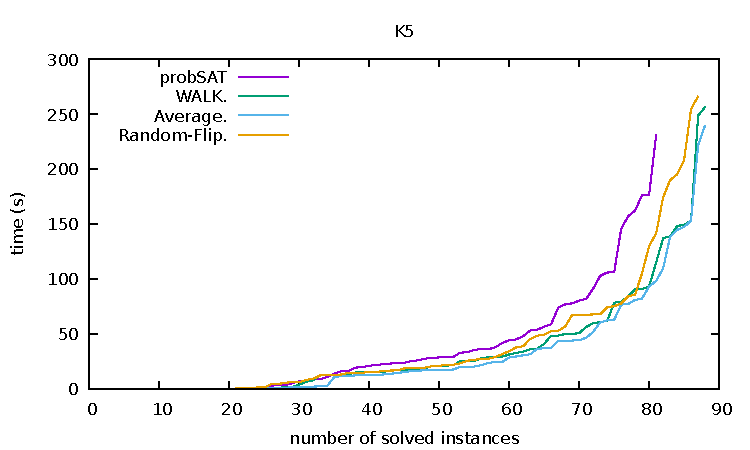
\includegraphics[scale = 0.8]{DATA/K5/e4.pdf}
  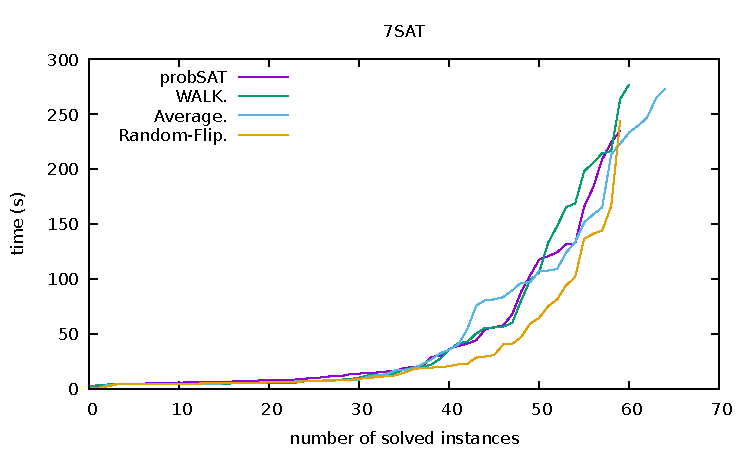
\includegraphics[scale = 0.8]{DATA/K7/e4.pdf}
  \end{center}
  \label{Experiment 9 k3 cactus plot}
  \end{figure}
  \begin{figure}[H]
\begin{center}

  \end{center}
  \caption{Our variants can get better performances and efficiencies for 3SAT and 5SAT problems in whole process. For 7SAT oroblems, our variants can solve more problems than the original \emph{probSAT}. }
  \label{Experiment 9 k5 cactus plot}
  \end{figure}
  \clearpage
  \subsubsection{Experiment 5: The pure portfolio approach} 
  \label{sec:Experiment 5}
Our parallel implementation uses OpenMP to support shared memory multiprocessing. In our local \emph{C++} Implementation, we use the function \emph{rand}() in the standard library to generate pseudo-random integer. This function is not thread-safe. To implement a deterministic parallel implementation, we use \emph{rand}()  for in the first thread and use the thread safe random engine in \emph{C++} for random value generation for other threads. Based on the observation in our experiments, the sequential implementation with the simple \emph{rand}() function has the best performance for the whole set. For most problems, some random value generators can search following a valid search path to a satisfying assignment. But there is no one random generator that are advantages for all the problems. This approach takes advantage of the performances differences of random generator. The threads execute the swpSAT with different random engine in parallel. If one thread find a satisfying assignment,the whole parallel search can stop. With our experiment, the parallel search gets a performance like the minimum runtime of one-thread local search with different random value engines. \\
\begin{table}[h!]
\begin{center}
    \begin{tabular}{|l|l|l|l|l|p{1cm}|}
\hline 
$rand()$&$minstd\_rand$&$mt19937$\\ \hline
$mt19937\_64$&$ranlux24\_base$&$ranlux48\_base$\\ \hline
$ranlux24$&$ranlux48$&$knuth\_b$\\ \hline
$default\_random\_engine$&$minstd\_rand0$&-\\ \hline
\end{tabular}
\end{center}
\caption{Pseudo-random number generators in use}
\end{table} 
\begin{table}[h!]
\begin{center}
    \begin{tabular}{|l|l|l|l|l|p{1cm}|}
\hline 
$rand()$&$minstd\_rand$&$mt19937$\\ \hline
$mt19937\_64$&$ranlux24\_base$&$ranlux48\_base$\\ \hline
$ranlux24$&$ranlux48$&$knuth\_b$\\ \hline
$default\_random\_engine$&$minstd\_rand0$&-\\ \hline
\end{tabular}
\end{center}
\caption{Pseudo-random number generators in use}
\end{table} 

  \begin{figure}[H]
\begin{center}
  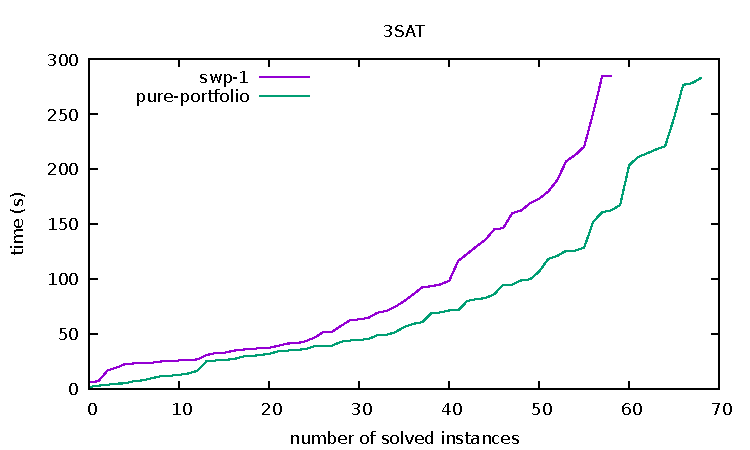
\includegraphics[scale = 0.8]{Parallel/K3/e1.pdf}
    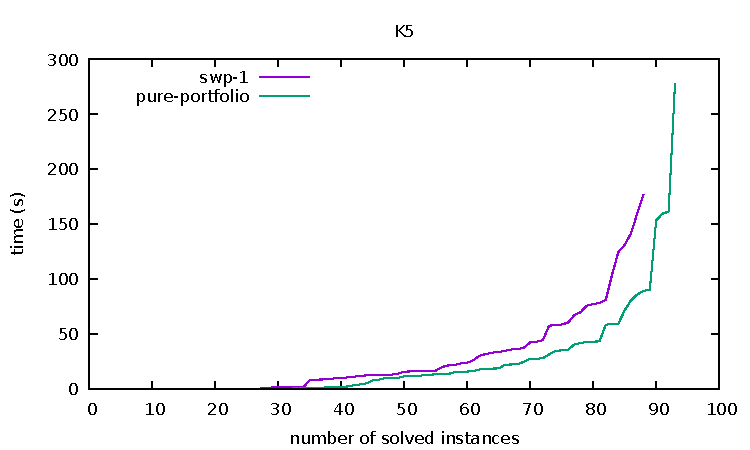
\includegraphics[scale = 0.8]{Parallel/K5/e1.pdf}
  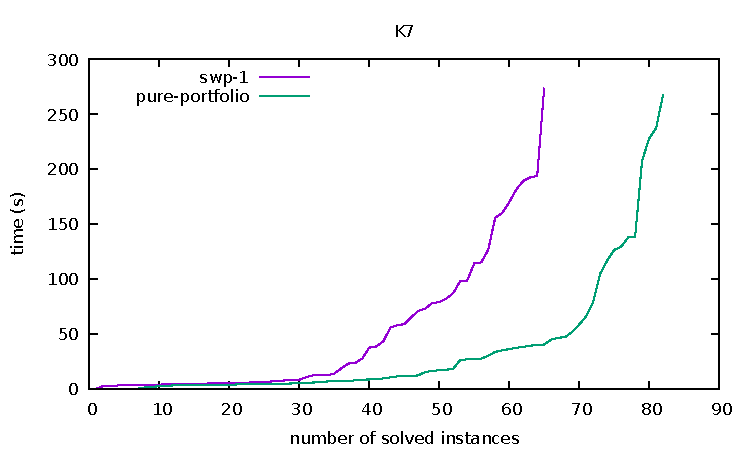
\includegraphics[scale = 0.8]{Parallel/K7/e1.pdf}
  \end{center}
    \label{Experiment 5 all cactus plot}
    \caption{The pure portfolio approach can get better performances and efficiencies in whole process. Expecially for 7SAT oroblems, the parallel solver  can solve $30\%$ more problems in same time. }
  \end{figure}
  \clearpage
\subsubsection{Experiment 6: Initialization with a guide of formula partitioning} 
\label{sec:Experiment 6}
\begin{table}[h!]
%\begin{minipage}{\textwidth}                                                                                         
\begin{center}
    \begin{tabular}{|l|l|l|l|l|p{1cm}|}
\hline 
    Solver &$3-3(big)$&$3-3(small)$&$3-5$&$5-5$&$5-7$\\ \hline
   	swpSAT &1861.73	&7955.19 &-	&2748.13&-\\ \hline
    FineInit& 501.78 (26.95\%)& 1734.79 (21.81\%) &-&621.47(22.61\%)&- \\ \hline
     \hline
    Solver & $7-7$ & BIG & SMALL & COMBINE &\\ \hline
    swpSAT &3276.39	&	2794.15 &15579.71& 18373.86&\\ \hline
    FineInit&376.06 (11.48\% )&902.69(32.31\%) & 3099.02(19.89\%)&4001.71(21.78\%)&\\ \hline
\end{tabular}
\end{center}
%\end{minipage}
\end{table} 

 \begin{figure}[H]
\begin{center}
  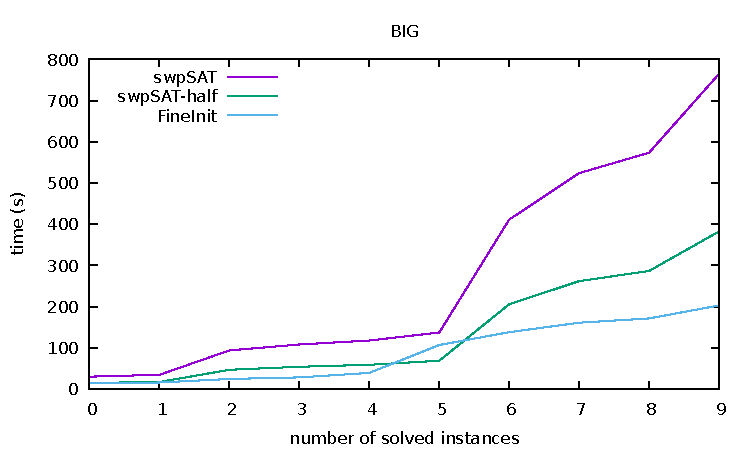
\includegraphics[scale = 1]{DATA/BIG/a4.pdf}
    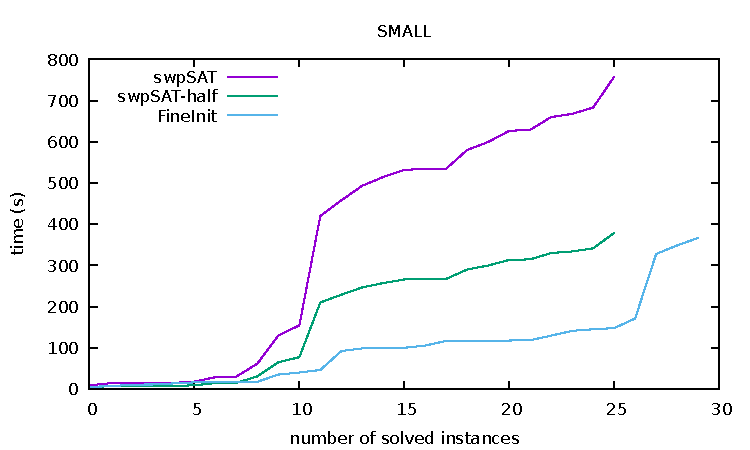
\includegraphics[scale = 1]{DATA/SMALL/a4.pdf}
    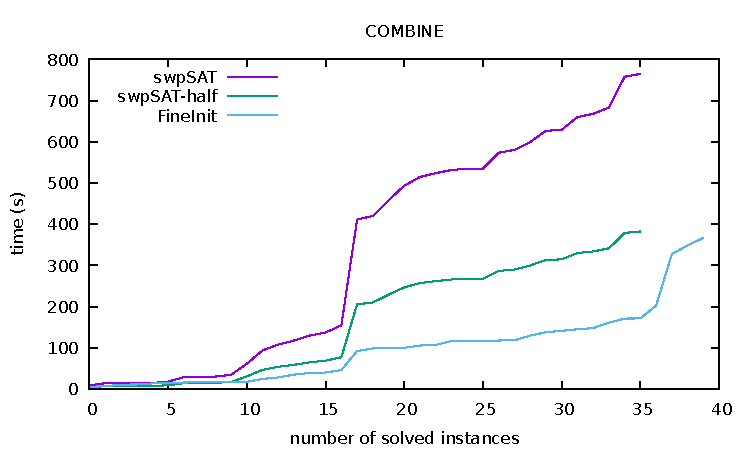
\includegraphics[scale = 1]{DATA/COMBINE/a4.pdf}
  \end{center}
  \caption{}
  \label{Experiment 6 COMBINE}
  \end{figure} 
\clearpage
\subsubsection{Experiment 7:2017-UNIF Comparision (parallel)} 
\label{sec:Experiment 7}

 \begin{figure}[H]
\begin{center}
  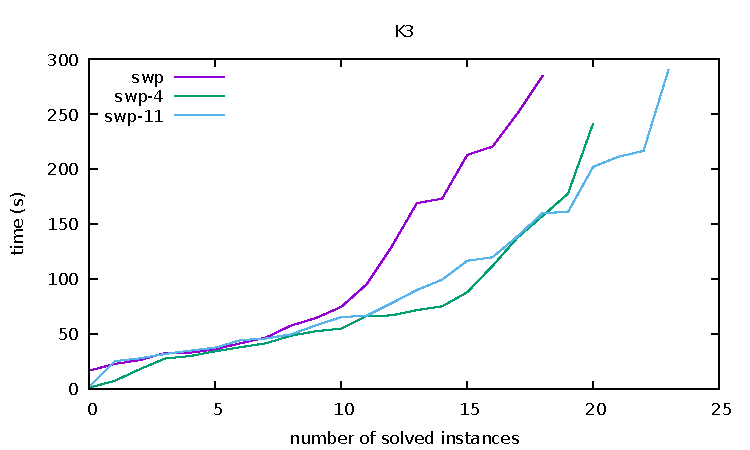
\includegraphics[scale = 0.8]{Parallel/K3/e2.pdf}
    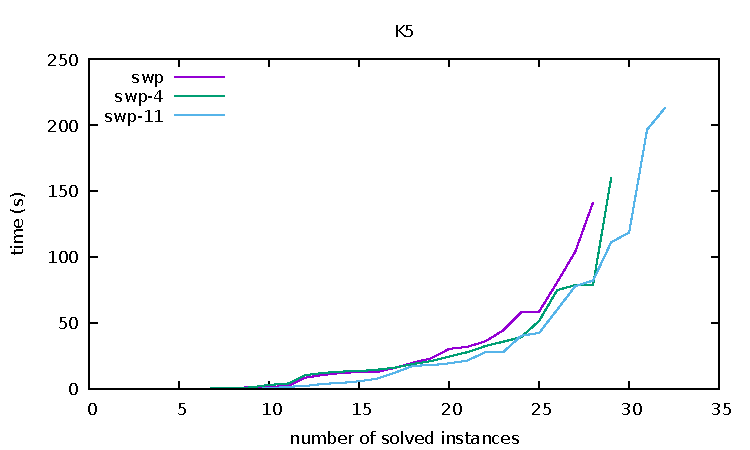
\includegraphics[scale = 0.8]{Parallel/K5/e2.pdf}
  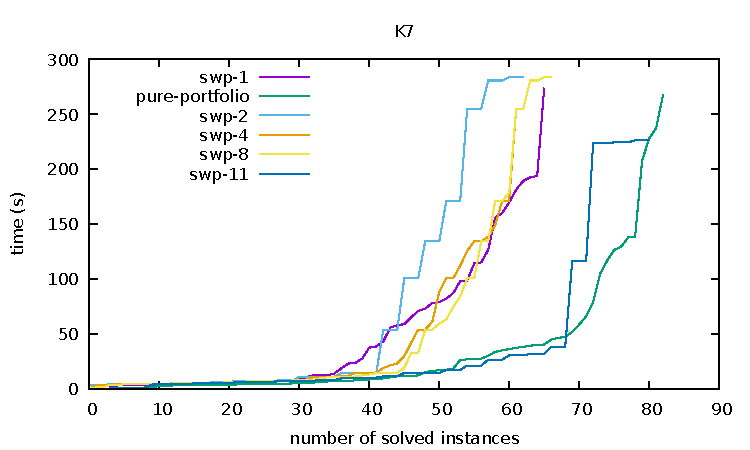
\includegraphics[scale = 0.8]{Parallel/K7/e2.pdf}
  \end{center}
  \caption{}
  \label{Experiment 6 COMBINE}
  \end{figure}
\clearpage
\section{Conclusion}

\label{sec:conc}
Local search is a universally applicable approach to solve random SAT problems. We present a stochastic local search algorithm with the cooperation of \emph{walkSAT} and \emph{probSAT}.\\
\\
In section 3, we discussed the basic scheme of our sequential algorithm. In, we compare the original \emph{probSAT} with a randomly generated initial solution and our version based on the occurrence of os literals in formel. Based on our experiment, our initialization is advantages n the number of solved problems and also in the execution time of the search. To get the advantage of the greedy algorithm and use the robustness of the stochastic process, we introduce the data structure statistic list to guide the decision between these two processes in step $pickVar()$. Here we propose some variants to make the distinction between greedy choice and a random choice. Generally, our local searches get better performance than the \emph{probSAT} algorithm. \\
Based on the performance of these searches in kSAT problems, we get our swpSAT solver, which combines the advantages of the local searches. \\
\\
In section 4, we make our swpSAT solver parallel with different approaches. Most problems get similar results with the different seed of one random generator. However, the formulas get different results with different random generation. With this fact, we make the parallel version of our local search, in which the agents run the search with different random generators and then take advantages of the suitable one.\\
In the following part of this section, we discussed the combination of formula partitioning and our parallel solver. After trying several approaches with failure, we found the way of using formula partitioning to make a fine initial solution save search time and furthermore solve more problems. Our experiments evaluate the hyperthesis that the formula partitioning information can guide the local search and improve the efficiency in the parallel search.
\subsection{Further work}
\clearpage
\section{Bibliography}
\bibliographystyle{ieeetr}
\bibliography{references}
\end{document}
